%%
%% (
%%  )\ )                             (
%%  (()/(   (            (             )\  )   (
%%   /(_))  ))\   (       ))\  (   (   (()/(   ))\
%%   (_))  /((_)  )\  )  /((_) )\  )\   ((_))/((_)
%%   | _ \(_))(  _(_/( (_) )  ((_)((_)  _| |(_))
%%   |   /| || || ' \))/ -_)/ _|/ _ \/ _` |/ -_)
%%   |_|_\ \_,_||_||_| \___|\__|\___/\__,_|\___|
%%

\documentclass{article}
\usepackage[utf8x]{inputenc}
\usepackage{amsmath}
%\usepackage{slashbox}
\usepackage{amsfonts}
\usepackage{amssymb}
\usepackage{graphicx} % Paquete para incluir imágenes en el documento LaTeX
\usepackage{hyperref}
\hypersetup{
  colorlinks=true,
  linkcolor=blue,
  filecolor=magenta,
  urlcolor=cyan,
}
\urlstyle{same}
\usepackage{varwidth}

\newcommand\tab[1][1cm]{\hspace*{#1}}

\usepackage{multirow}

\usepackage[a4paper,rmargin=1.5cm,lmargin=1.5cm,top=1.5cm,bottom=1.5cm]{geometry}

\usepackage{pdfpages}

\usepackage{xcolor}
\usepackage{minted}
\setminted[cpp]{frame=lines, framesep=2mm, baselinestretch=1.2, rulecolor=\color{black!80},
                bgcolor=DarkGray,fontsize=\normalsize}
\usemintedstyle[cpp]{monokai}
\setminted[python]{frame=lines, framesep=2mm, baselinestretch=1.2, rulecolor=\color{black!80}, bgcolor=DarkGray}
\usemintedstyle[python]{monokai}
\setminted[java]{frame=lines, framesep=2mm, baselinestretch=1.2, rulecolor=\color{black!80}, bgcolor=DarkGray}
\usemintedstyle[java]{monokai}
\setminted[javascript]{frame=lines, framesep=2mm, baselinestretch=1.2, rulecolor=\color{black!80}, bgcolor=DarkGray}
\usemintedstyle[javascript]{monokai}
\setminted[php]{frame=lines, framesep=2mm, baselinestretch=1.2, rulecolor=\color{black!30}, bgcolor=LightGray}
\setminted[html]{frame=lines, framesep=2mm, baselinestretch=1.2, rulecolor=\color{black!30}, bgcolor=LightGray}
\setminted[bash]{baselinestretch=1.2,rulecolor=\color{black!30},fontsize=\footnotesize,bgcolor=LightGray}
\definecolor{LightGray}{gray}{0.98}
\definecolor{DarkGray}{gray}{0.1}
\definecolor{MidGray}{gray}{0.8}
\definecolor{codegreen}{rgb}{0,0.6,0}
\definecolor{codegray}{rgb}{0.5,0.5,0.5}
\definecolor{codepurple}{rgb}{0.58,0,0.82}
\definecolor{backcolour}{rgb}{0.95,0.95,0.92}

\setlength{\parindent}{0px}  % Setea la indentacion de la primera linea de cada parrafo a cero pixeles.


\title{Curso de Programación Orientada a Objetos: POO}
\author{@RuneCode}

\begin{document}
%% Portada
\includepdf{./portada/portada.pdf}

%% Clase 1
\section{Instalando Visual Studio Code}%
Visual Studio Code es un editor bastante ligero que puede trabajar con muchos
lenguajes de programación simultáneamente. Lo puedes encontrar en las tres
versiones básicas de Sistema Operativo (Windows, Mac y Linux) y lo puedes
descargar directo en este
\href{https://code.visualstudio.com/download}{enlace}.\\

Cuando la instalación haya terminado, verás algo como esto:

\begin{figure}[h!]
  \centering
  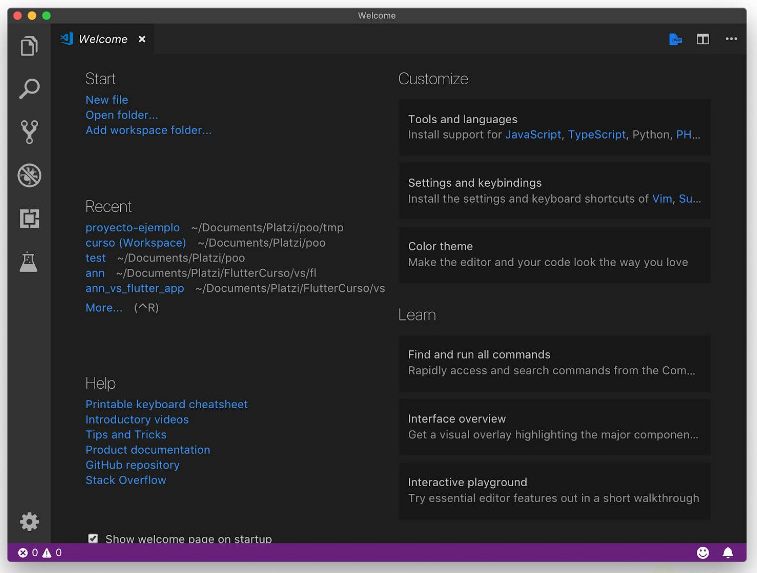
\includegraphics[scale=0.65]{./Pictures/022_vscode.png}
\end{figure}

Ahora pasameo a configurarlo para cada lenguaje.\\

Primero ubica la sección \textbf{Extensiones} o en inglés \textbf{Extensions},
además de la barra de Search porque estaremos buscando la extensión para cada
lenguaje.

\begin{figure}[h!]
  \centering
  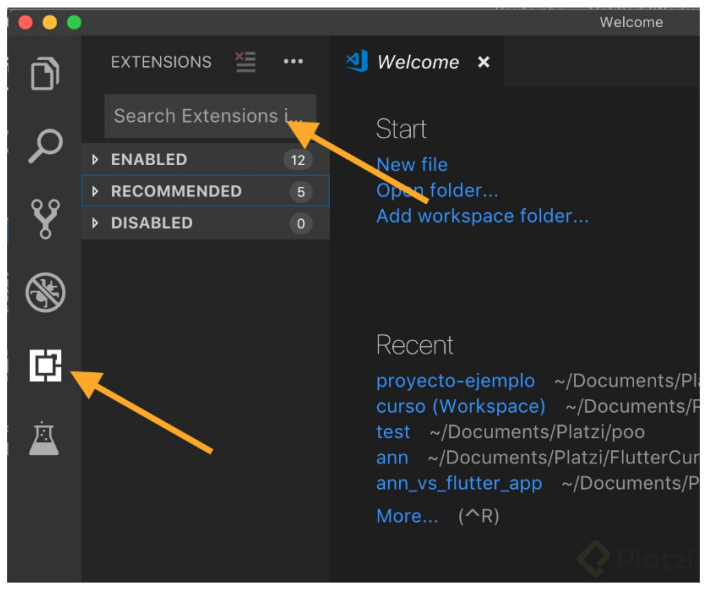
\includegraphics[scale=0.65]{./Pictures/023_vscode.png}
\end{figure}

\newpage
\textbf{Java}\\
En la barra de Search Extensions escribe: \textbf{Java Extension Pack} y da clic
en el botón verde \textbf{Install}.

\begin{figure}[h!]
  \centering
  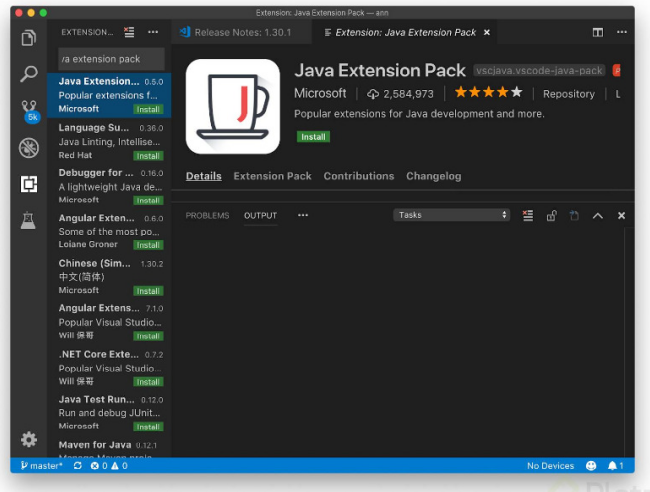
\includegraphics[scale=0.75]{./Pictures/024_vscode.png}
\end{figure}

Ahora, para tener una mejor experiencia en Debugging, instala el Debbuger for
Java, el cual encuentras siguiendo el procedimiento anterior.

\begin{figure}[h!]
  \centering
  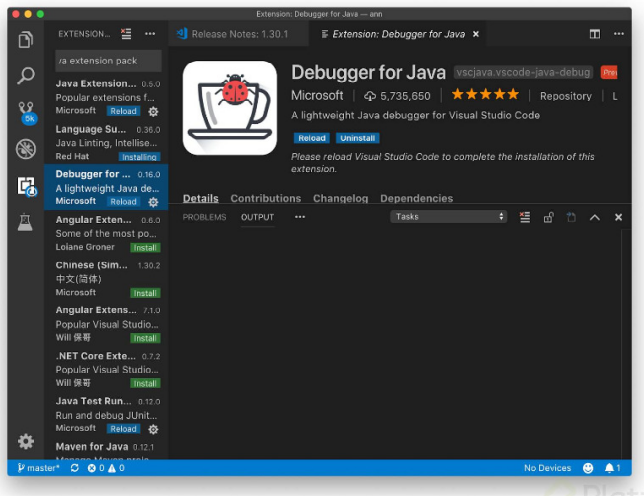
\includegraphics[scale=0.75]{./Pictures/025.png}
\end{figure}

Listo, terminamos con Java. Ahora vamos por Python.\\

\newpage
\textbf{Python}\\
Comencemos instalando Python en nuestra computadora. Dirígete al sitio
\href{https://www.python.org/}{python.ogr}  y dale clic al botón de Descargar.

\begin{figure}[h!]
  \centering
  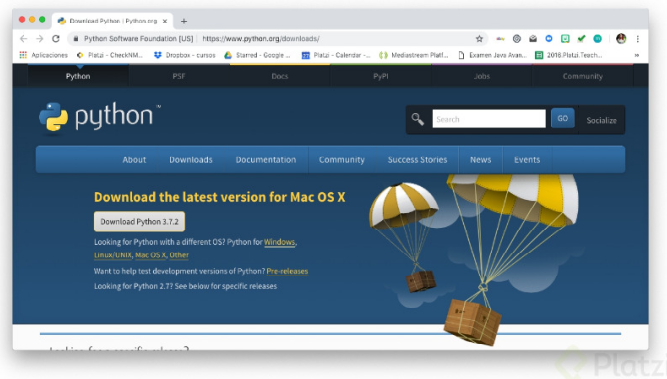
\includegraphics[scale=0.75]{./Pictures/026_python.png}
\end{figure}

Ve de la mano con el asistente hasta finalizar la instalación.

\begin{figure}[h!]
  \centering
  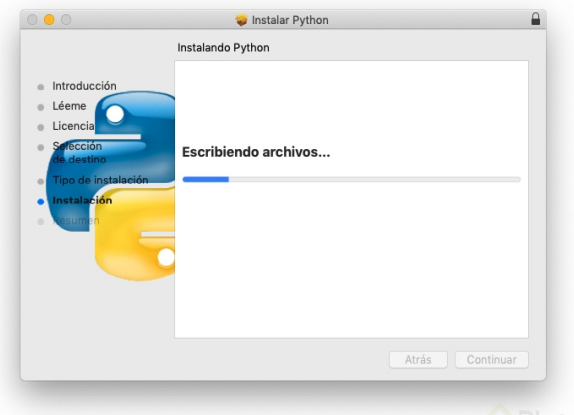
\includegraphics[scale=0.75]{./Pictures/027_python.png}
\end{figure}


Ahora prosigamos con PHP.\\

\newpage
\textbf{PHP}\\

Para configurar PHP buscaremos la extensión \textbf{PHP Server} y pulsamos Inslatar.

\begin{figure}[h!]
  \centering
  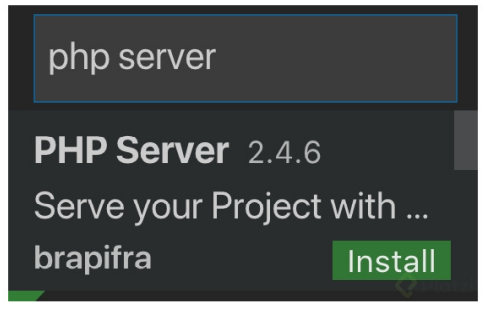
\includegraphics[scale=0.35]{./Pictures/028_php_server.png}
\end{figure}

\textbf{JavaScript}\\

En este caso no necesitamos instalar absolutamente nada, utilizaremos el editor
con su configuración por defecto.\\

\textbf{Comencemos nuestro proyecto}\\

Ya está todo listo, ahora dejemos creado el proyecto.\\
Para esto seleccionaremos la opción \textbf{Add workspace folder}.

\begin{figure}[h!]
  \centering
  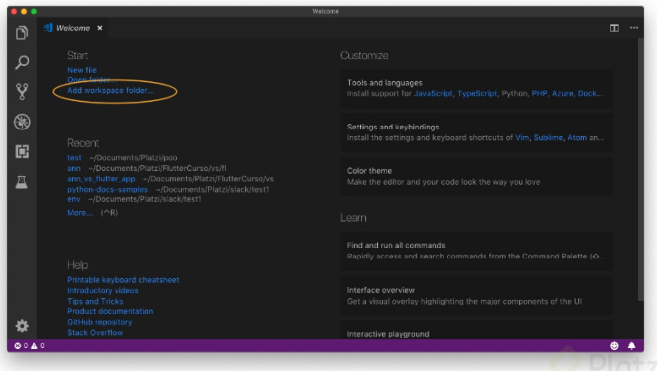
\includegraphics[scale=0.75]{./Pictures/029_workspace.png}
\end{figure}

A continuación creamos una carpeta llamada \textbf{CursoPOOUber} y damos clic
en Add para finalizar. Ahora generaremos esta estructura de carpetas para
manejar los documentos correspondientes al lenguaje de programación.

\begin{figure}[h!]
  \centering
  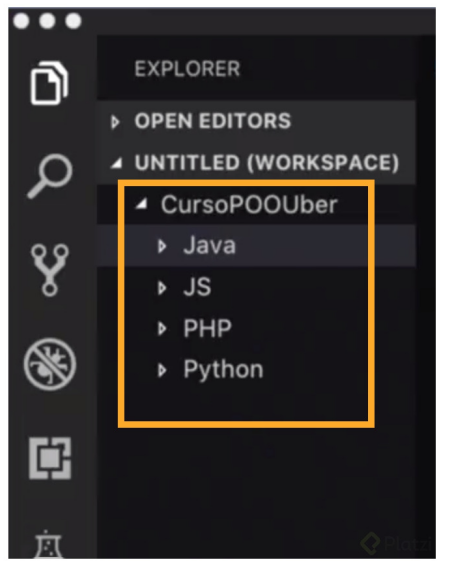
\includegraphics[scale=0.45]{./Pictures/030_carpetas.png}
\end{figure}

\newpage
Ahora que tenemos listo nuestro sistema de archivos terminemos la configuración
de Python en VSC, vamos al menú View -> Command Pallette y escribimos python
"Seleccionar intérprete", tal como se muestra en la figura.\\

\begin{figure}[h!]
  \centering
  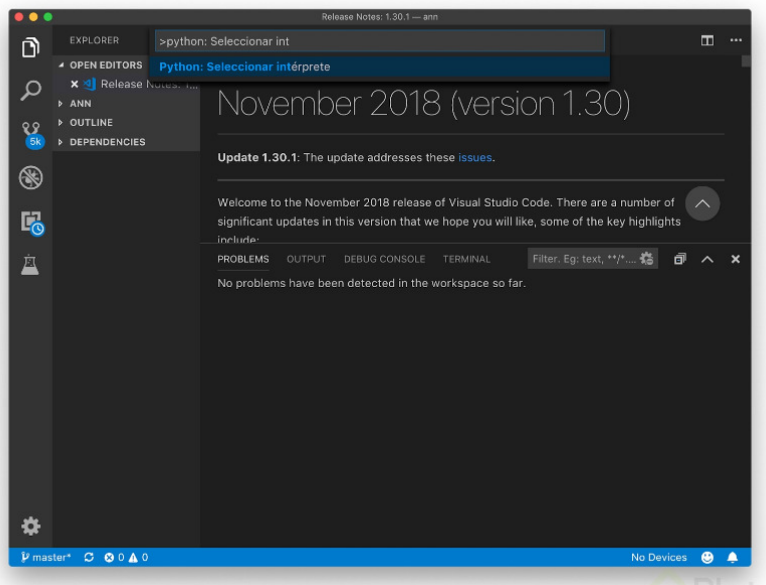
\includegraphics[scale=0.75]{./Pictures/031_python_interprete.png}
\end{figure}

%% Clase 2
\section{¿Por qué aprender Programación Orientada a Objetos?}%
\textbf{Vas a programar más rápido}. Tener un análisis previo de lo que estás
realizando te ayudará a generar código mucho más veloz.\\
\textbf{Dejas de ser Programador Jr.} Podrás responder preguntas como ¿Qué es
encapsulamiento?, ¿Qué es Abstracción?, ¿Qué es Herencia?, ¿Qué es
Polimorfismo? en futuras entrevistas de trabajo.\\
\textbf{Dejar de Copiar y Pegar Código}.

%% Clase 3
\section{¿Qué resuelve la Programación Orientada a Objetos?}%
La programación Orientada a Objetos nace de los problemas creados por la
programación estructurada y nos ayuda a resolver ciertos problemas como:\\
\begin{itemize}
  \item Código muy largo: A medida que un sistema va creciendo y se hace más
    robusta el código generado se vuelve muy extenso haciéndose difícil de
    leer, depurar, mantener.
  \item Si algo falla, todo se rompe: Ya que con la programación estructurada
    el código se ejecuta secuencialmente al momento de que una de esas líneas
    fallara todo lo demás deja de funcionar.
  \item Difícil de mantener.
\end{itemize}

\newpage
%% Clase 4
\section{Paradigma Orientado a Objetos}%
La \textbf{Programación Orientada a Objetos} viene de una filosofía o forma de
pensar que es la Orientación a Objetos y esto surge a partir de los problemas
que necesitamos plasmar en código.\\

Es analizar un problema en forma de objetos para después llevarlo a código, eso
es la \textbf{Orientación a Objetos.}\\

Un \textbf{paradigma} es una teoría que suministra la base y modelo para
resolver problemas. El paradigma de Programación Orientado a Objetos se compone
de 4 elementos.

\begin{itemize}
  \item Clases
  \item Propiedades
  \item Métodos
  \item Objetos
\end{itemize}

Y 4 pilares:

\begin{itemize}
  \item Encapsulamiento
  \item Abstracción
  \item Herencia
  \item Polimorfismo
\end{itemize}

%% Clase 5
\section{Lenguajes Orientados a Objetos}%
Algunos de los lenguajes de programación Orientados a Objetos son:
\begin{itemize}
  \item Java
  \item PHP
  \item Python
  \item JavaScript
  \item C\#
  \item Ruby
  \item Kotlin
\end{itemize}

\subsection*{Java}%
Es un lenguaje Orientado a Objetos naturalmente, es muy usado en el desarrollo
movil en Android y también en la parte del Servidor (Backend: API Rest, Spring,
Hybernate). Los archivos se identificarán con la extensión \textbf{.java}.

\subsection*{PHP}%
PHP es un lenguaje interpretado pensado para la Web, lo interpreta el
navegador. Los archivos se indentificarán con la extensión \textbf{.php}.

\subsection*{Python}%
Diseñado para ser fácil de usar compitiendo en este aspecto con Ruby, pero 
con una comunidad mucho más grande. Tiene múltiples usos: Web, Server Side,
Análisis de Datos, Machine Learning, etc. Los archivos se identificarán con la
extensión \textbf{.py}

\subsection*{JavaScript}%
Es un lenguaje interpretado, Orientado a Objetos pero basado en prototipos.
Pensado para la Web aunque también se pueden ejecutar en el lado del servidor
con node. Los archivos que trabajaremos con JavaScript serán archivos con
extensión \textbf{.js}.

\subsection*{Entorno de Desarollo}%
Visual Studio Code es un Entorno de Desarrollo que permite manejar muchos
lenguajes de programación.


%% Clase 6
\section{Diagramas de Modelado}%

\textbf{OMT}: Object Modeling Techniques. Es una metodología para el análisis
orientado a objetos.\\

\textbf{UML}: Unified Modeling Language. Tomó las bases y técnicas de OMT
unificándolas. Tenemos más opciones de diagramas como lo son: Clases, Casos de
uso, Objetos, Actividades, Iteración, Estados, Implementación.

%% Clase 7
\section{UML}%
UML significa Unified Modeling Language el cual es un lenguaje estándar de
modelado de sistemas orientados a objetos.

\begin{figure}[h!]
  \centering
  
\includegraphics[scale=0.75]{./Pictures/001_UML.png}
\end{figure}

Tenemos los siguientes elementos que se representan de la siguiente manera:

Las \textbf{clases} se representan así:

\begin{figure}[h!]
  \centering
  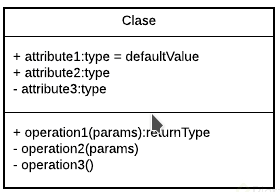
\includegraphics[scale=0.75]{./Pictures/002_clase.png}
\end{figure}

En la parte superior se colocan los atributos o propiedades, y debajo las
operaciones de la clase. Notarás que el primer carácter con el que empiezan es
un símbolo. Este denotará la visibilidad del atributo o método, esto es un
término que tiene que ver con Encapsulamiento y veremos más adelante a detalle.\\

Estos son los niveles de \textbf{visibilidad} que puedes tener:
\begin{itemize}
  \item {-} private
  \item + public
  \item \# protected
  \item \textasciitilde{} default
\end{itemize}


Una forma de representar las relaciones que tendrá un elemento con otro es a
través de las flechas en UML, y aquí tenemos varios tipos, estos son los más
comunes:\\

\textbf{Asociación}\\

\begin{figure}[h!]
  \centering
  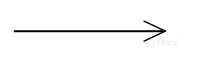
\includegraphics[scale=0.75]{./Pictures/003_asociacion.png}
\end{figure}

Como su nombre lo dice, notarás que cada vez que esté referenciada este tipo de
flecha significará que ese elemento contiene al otro en su definición. La flecha
apuntará hacia la dependencia.

\begin{figure}[h!]
  \centering
  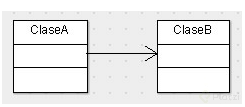
\includegraphics[scale=0.75]{./Pictures/004_asociacion.png}
\end{figure}

Con esto vemos que la ClaseA está asociada y depende de la ClaseB\\

\textbf{Herencia}\\

\begin{figure}[h!]
  \centering
  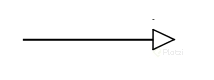
\includegraphics[scale=0.75]{./Pictures/005_herencia.png}
\end{figure}

Siempre que veamos este tipo de flechas se estará expresando la herencia. La
dirección de la flecha irá desde el hijo hasta el padre.\\

\begin{figure}[h!]
  \centering
  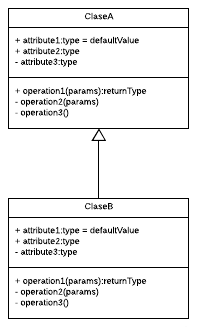
\includegraphics[scale=0.75]{./Pictures/006_herencia.png}
\end{figure}

Con esto vemos que la ClaseB hereda de la ClaseA\\

\textbf{Agregación}\\

\begin{figure}[h!]
  \centering
  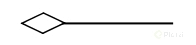
\includegraphics[scale=0.75]{./Pictures/007_agregacion.png}
\end{figure}

Este se parece a la asociación en que un elemento dependerá del otro, pero en
este caso será: Un elemento dependerá de muchos otros. Aquí tomamos como
referencia la multiplicidad del elelmento. Lo que comúnmente conocerías en Base
de Datos como Relaciones uno a muchos.

\begin{figure}[h!]
  \centering
  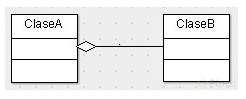
\includegraphics[scale=0.75]{./Pictures/008_agregacion.png}
\end{figure}

Con esto decimos que la ClaseA contiene varios elementos de la ClaseB. Estos
últimos son comúnmente representados con listas o colecciones de datos.\\

\textbf{Composición}

\begin{figure}[h!]
  \centering
  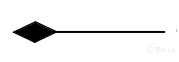
\includegraphics[scale=0.75]{./Pictures/009_composicion.png}
\end{figure}

Este es similar al anterior solo que su relación es totalmente compenetrada de
tal modo que conceptualmente una de estas class no podrían vivir si no
existiera la otra.

\begin{figure}[h!]
  \centering
  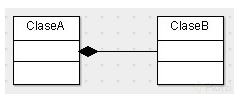
\includegraphics[scale=0.75]{./Pictures/010_composicion.png}
\end{figure}

Con esto terminamos nuestro primer módulo. Vamos al siguiente para entender
como podemos hacer un análisis y utilizar estos elementos para construir
nuestro diagrama de clases de Uber.


%% Clase 8
\section{Objetos}%
Los objetos son aquellos que tienen propiedades y comportamientos, también
serán sustantivos.\\

Pueden ser Físicos o Conceptuales:\\

La \textbf{Propiedades} tambiénn pueden llamarse atributos y estos también
serán sustantivos. Algunos atributos o propiedades son nombre, tamaño, forma,
estado, etc.\ son todas las características del objeto.\\

Los \textbf{Comportamientos} serán todas las operaciones que el objeto puede
hacer, suelen ser verbos o sustantivos y verbo. Algunos ejemplos pueden ser que
el usuario pueda hacer login y logout.

Nota: Es muy importante analizar el objeto dentro de su contexto.


%% Clase 9
\section{Abstracción y Clases}%
Una \textbf{Clase} es el modelo por el cual nuestros objetos se van a construir
y nos van a permitir generar más objetos.\\

Analizamos Objetos para crear \textbf{Clases}. Las \textbf{Clases} son los
modelos sobre los cuales construiremos nuestros objetos.\\

\textbf{Abstracción} es cuando separamos los datos de un objeto para generar un molde.

%% Clase 10
\section{Modularidad}%
La \textbf{modularidad} va muy relacionada con las clases y es un principio de
la Programación Orientado a Objetos y va de la mano con el Diseño Modular que
significa dividir un sistema en partes pequeñas y estas serán nuestros módulo
pudiendo funcionar de manera independiente.\\

La \textbf{modularidad} de nuestro código nos va a permitir.

\begin{itemize}
  \item Reutilizar
  \item Evitar colapsos
  \item Hacer nuestro código más mantenible
  \item Legibilidad
  \item Resolución rápida de problemas
\end{itemize}

Una buena práctica es separar las clases en archivos diferentes.

\newpage

%% Clase 11
\section{Analizando Uber en Objetos}%

\begin{figure}[h!]
  \centering
  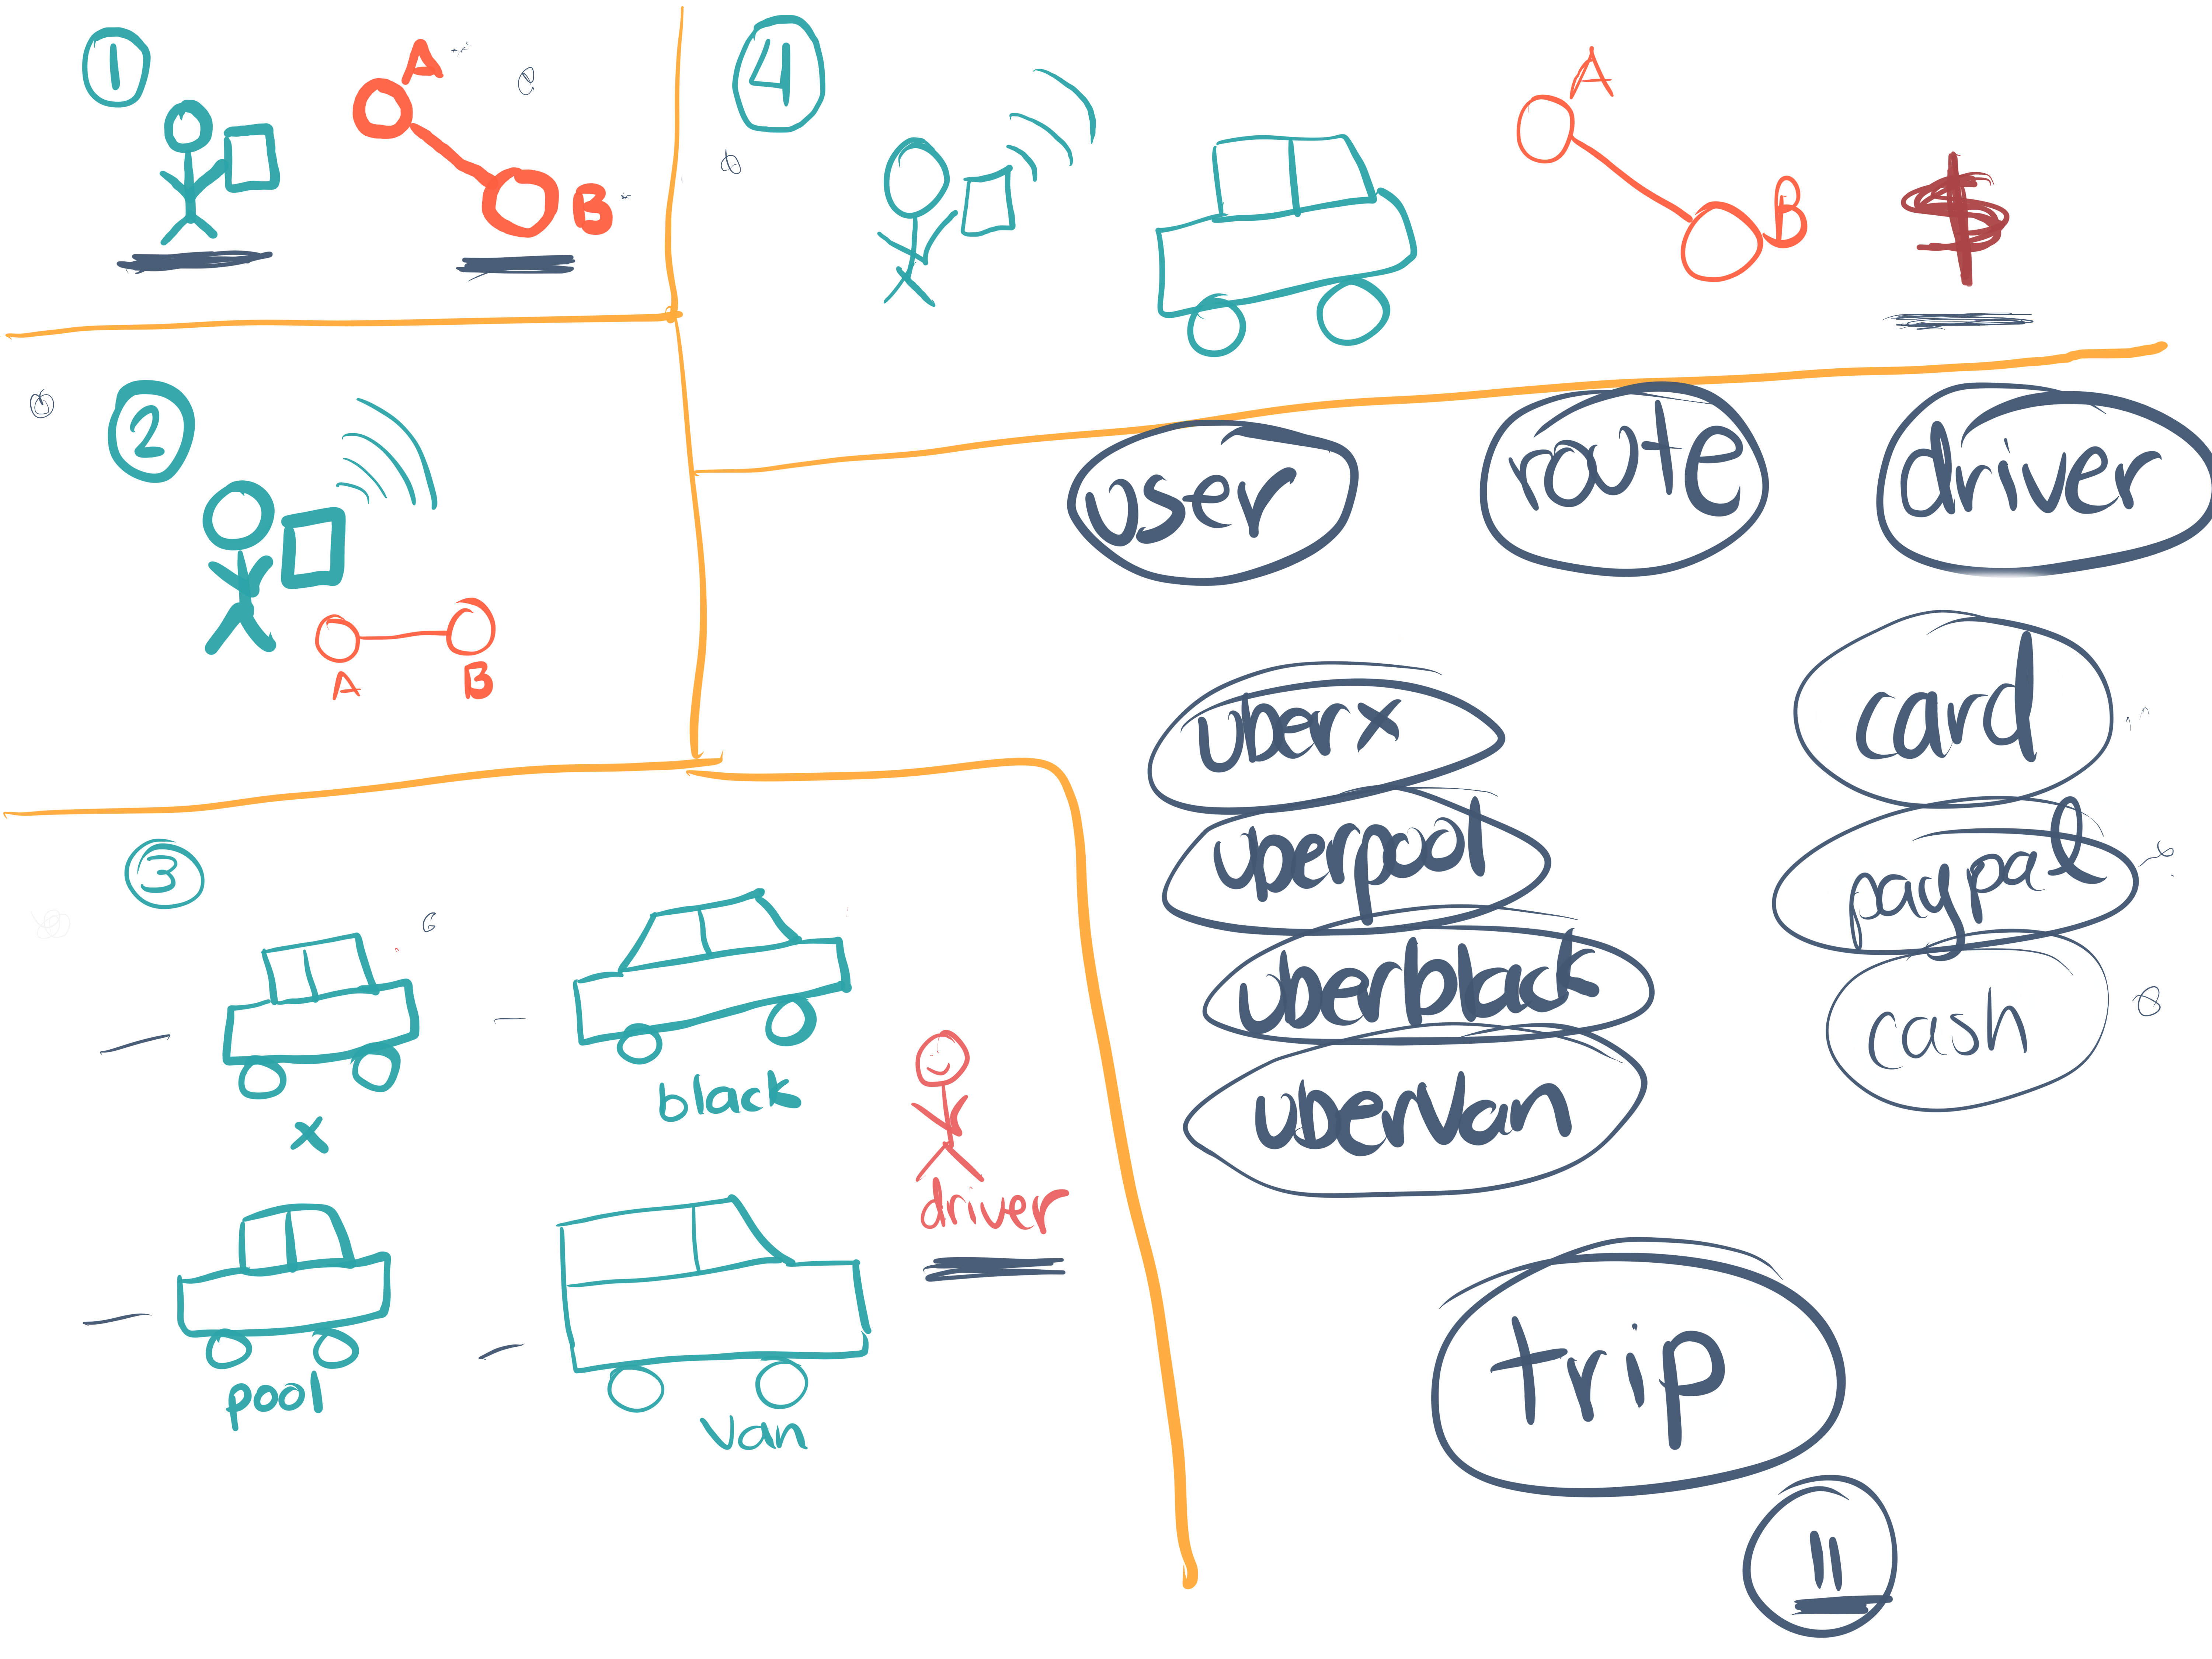
\includegraphics[scale=0.08]{./Pictures/011_uber_objetos.png}
\end{figure}


\newpage

%% Clase 12 - Reto 1: identificando objetos

%% Clase 13
\section{Modelando nuestros objetos Uber}%

\begin{figure}[h!]
  \centering
  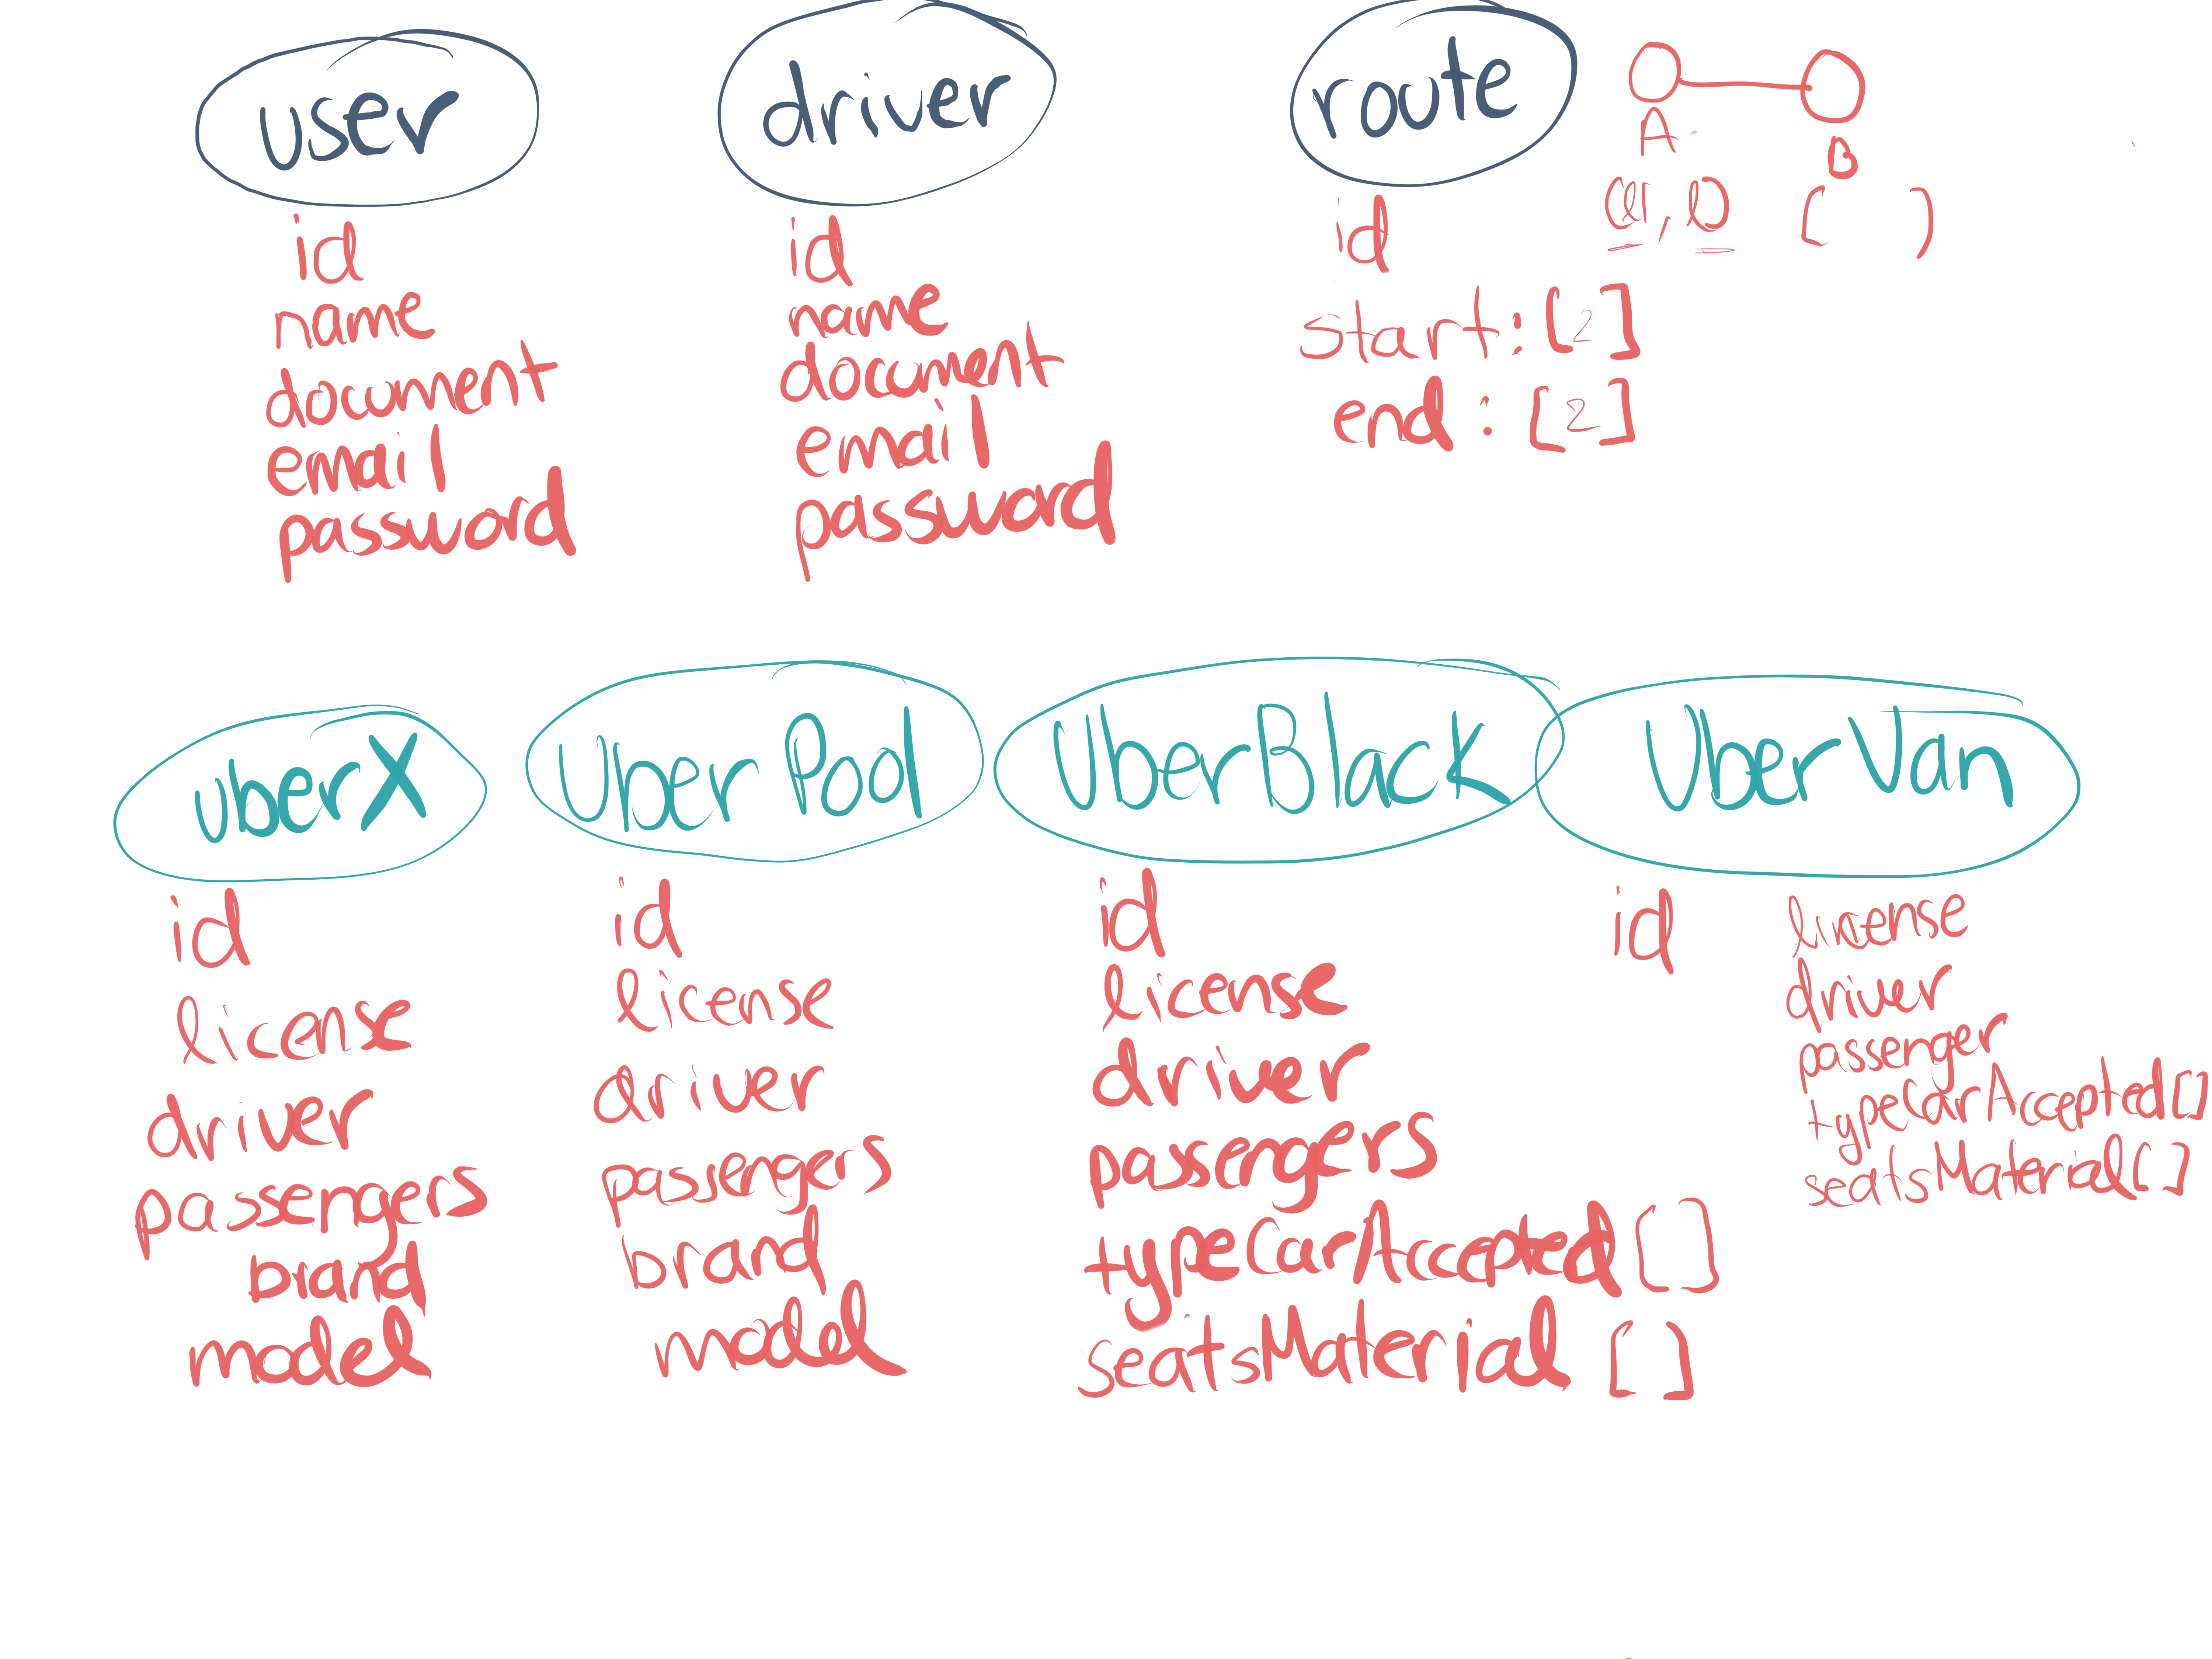
\includegraphics[scale=0.08]{./Pictures/012_modelando_objetos_uber.png}
\end{figure}

\begin{figure}[h!]
  \centering
  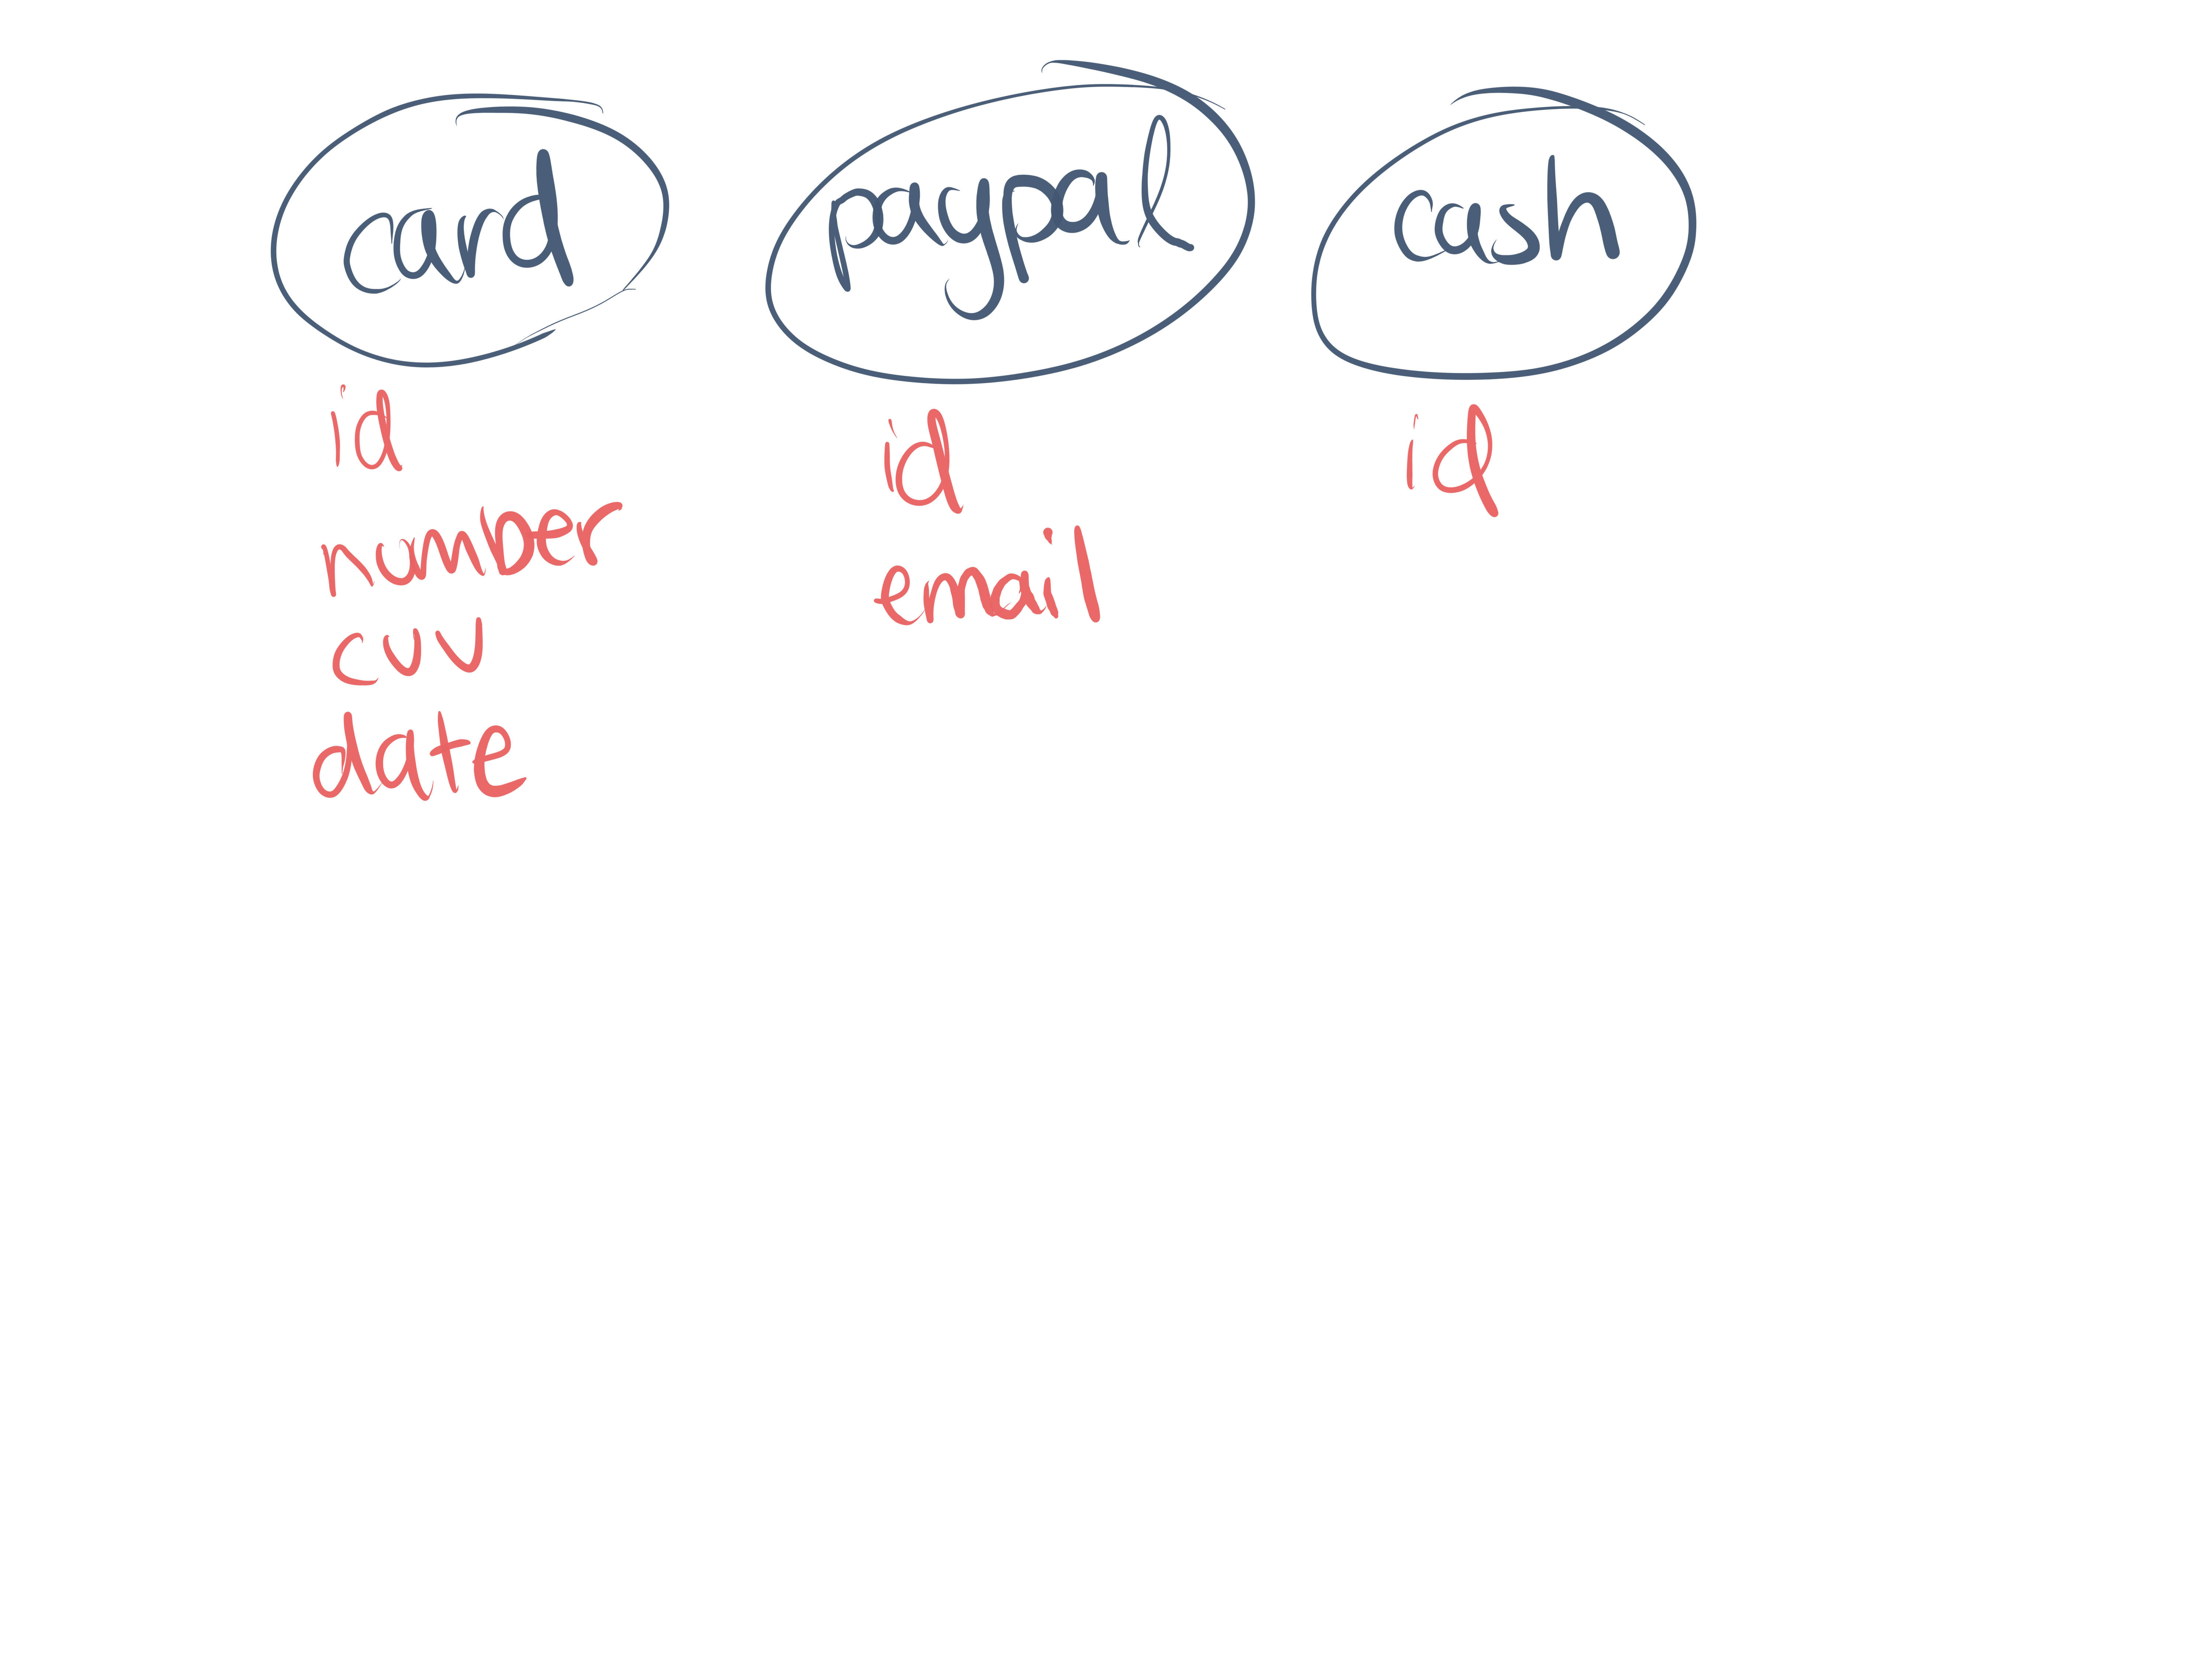
\includegraphics[scale=0.08]{./Pictures/013_modelando_objetos_uber.png}
\end{figure}

\newpage
%% Clase 14
\section{Clases en UML y su sintaxis en código}%

\textbf{Java}
\begin{minted}{java}
  class Person {
    String name = "";
    void walk(){}
  }
\end{minted}

\textbf{Python}
\begin{minted}{python}
  class Person:
    name = "";
    def walk():
\end{minted}

\textbf{Javascript}
\begin{minted}{javascript}
  function Person(){}
  Person.prototype.walk = function() {}
\end{minted}

\textbf{PHP}
\begin{minted}{php}
  <?php
  class Person {
    $name = "";
    function walk() {}
  }
  ?>
\end{minted}

%% Clase 15
\section{¿Qué es la herencia?}%
\textbf{Don't repeat yourself} es una filosofía que promueve la reducción de
duplicación en programación, esto nos va a inculcar que no tengamos líneas de
código duplicadas.\\

Toda pieza de información nunca debería ser duplicada debido a que incrementa
la dificultad en los cambios y evolución.\\

La \textbf{herencia} nos permite crear nuevas clases a partir de otras, se basa
en modelos y conceptos de la vida real. También tenemos una jerarquía de
\textbf{padre e hijo}.

\newpage
%% Clase 16
\section{Aplicando Herencia a nuestro proyecto Uber}%

\begin{figure}[h!]
  \centering
  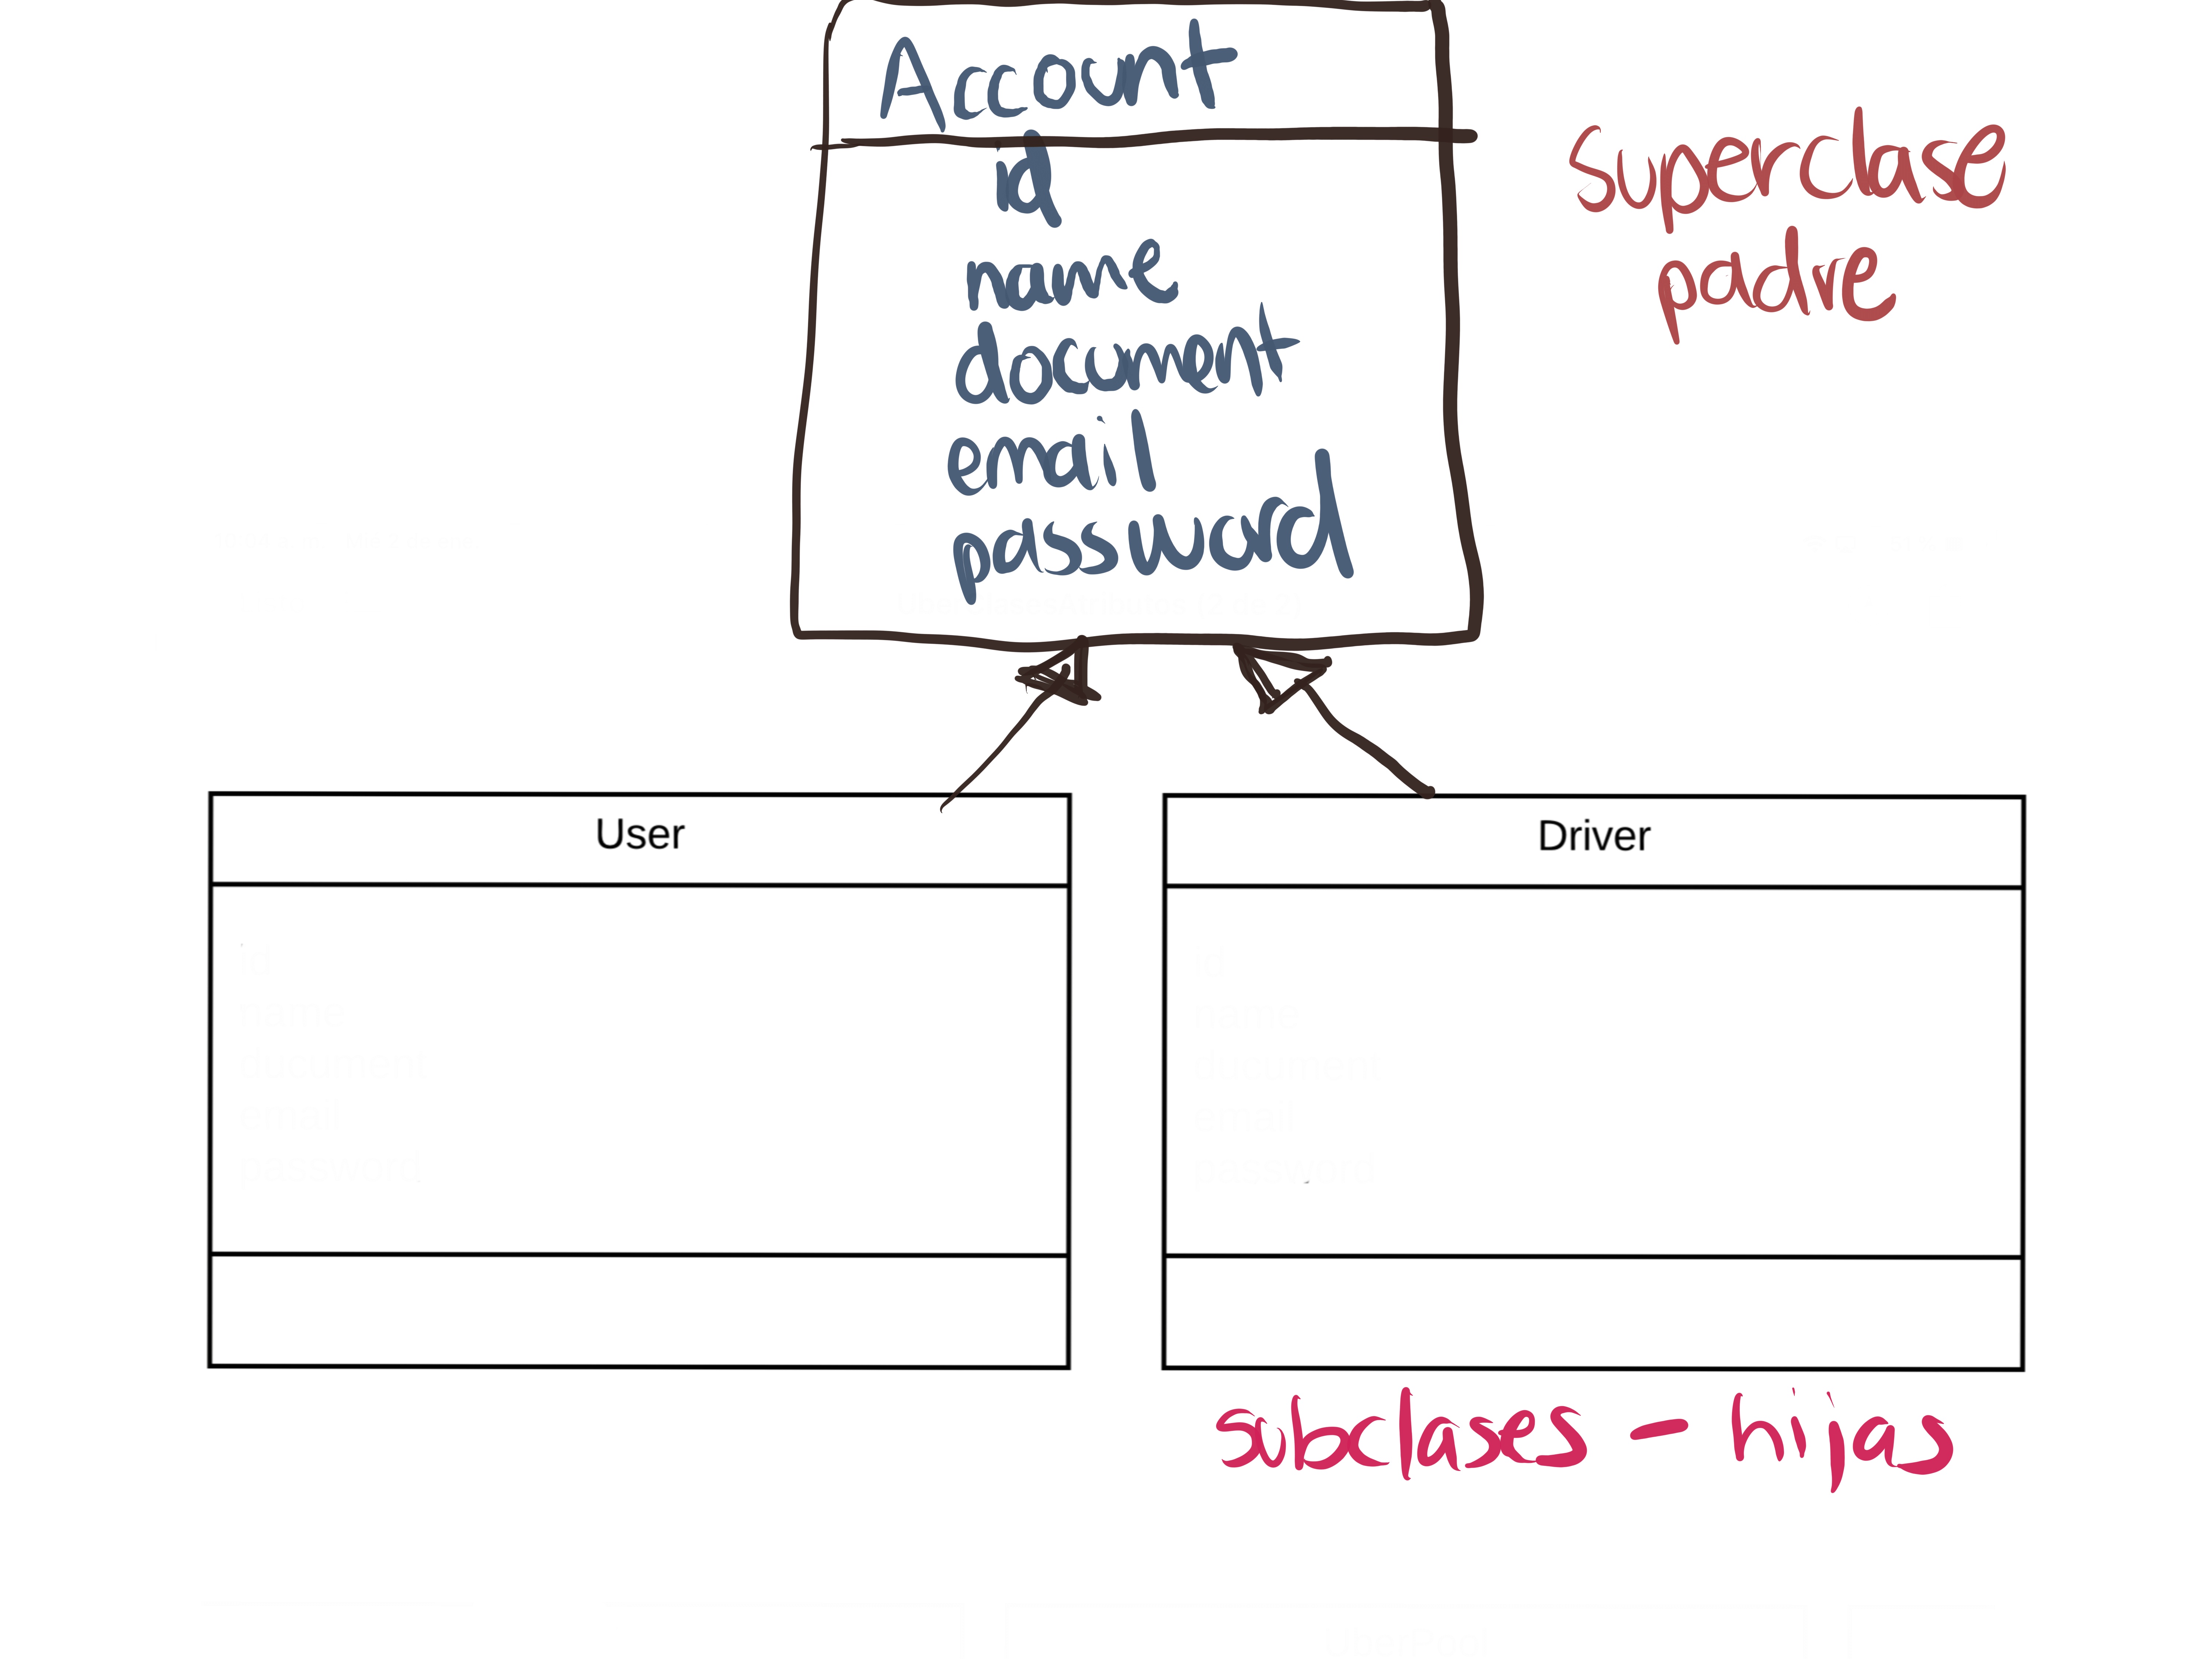
\includegraphics[scale=0.08]{./Pictures/014_herencia_proyecto_uber2.png}
\end{figure}

\begin{figure}[h!]
  \centering
  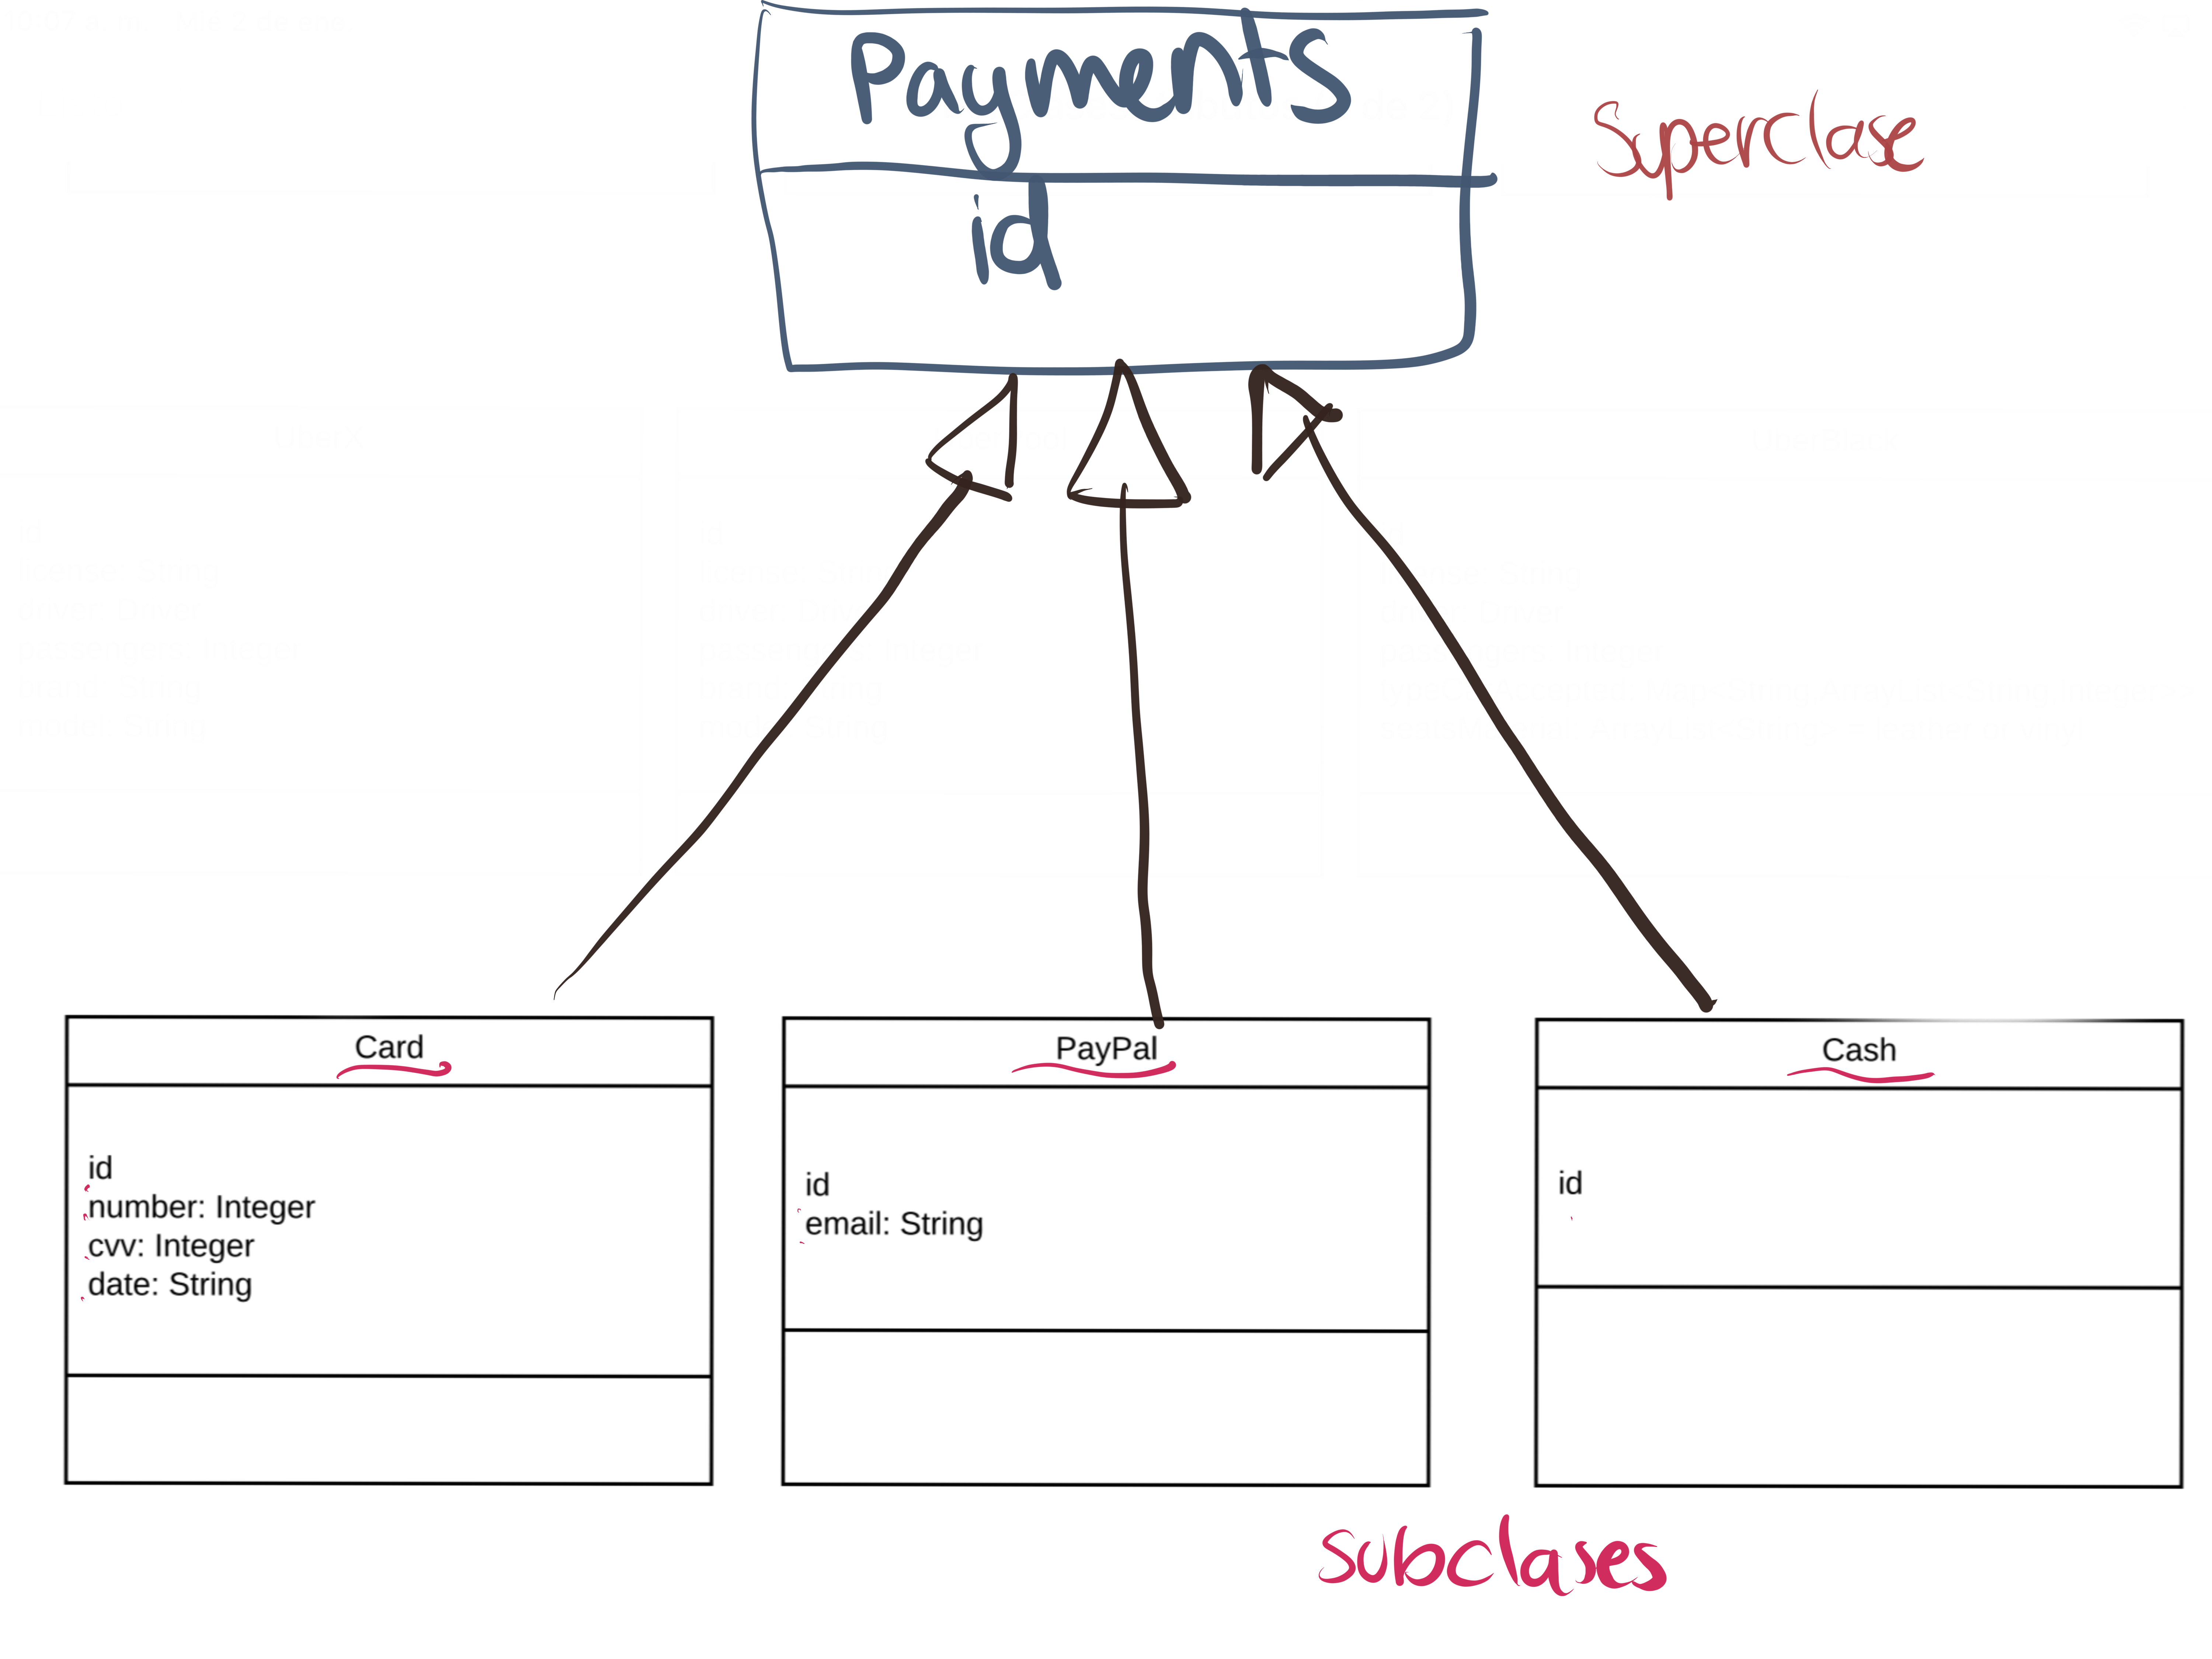
\includegraphics[scale=0.08]{./Pictures/015_herencia_proyecto_uber1.png}
\end{figure}

\begin{figure}[h!]
  \centering
  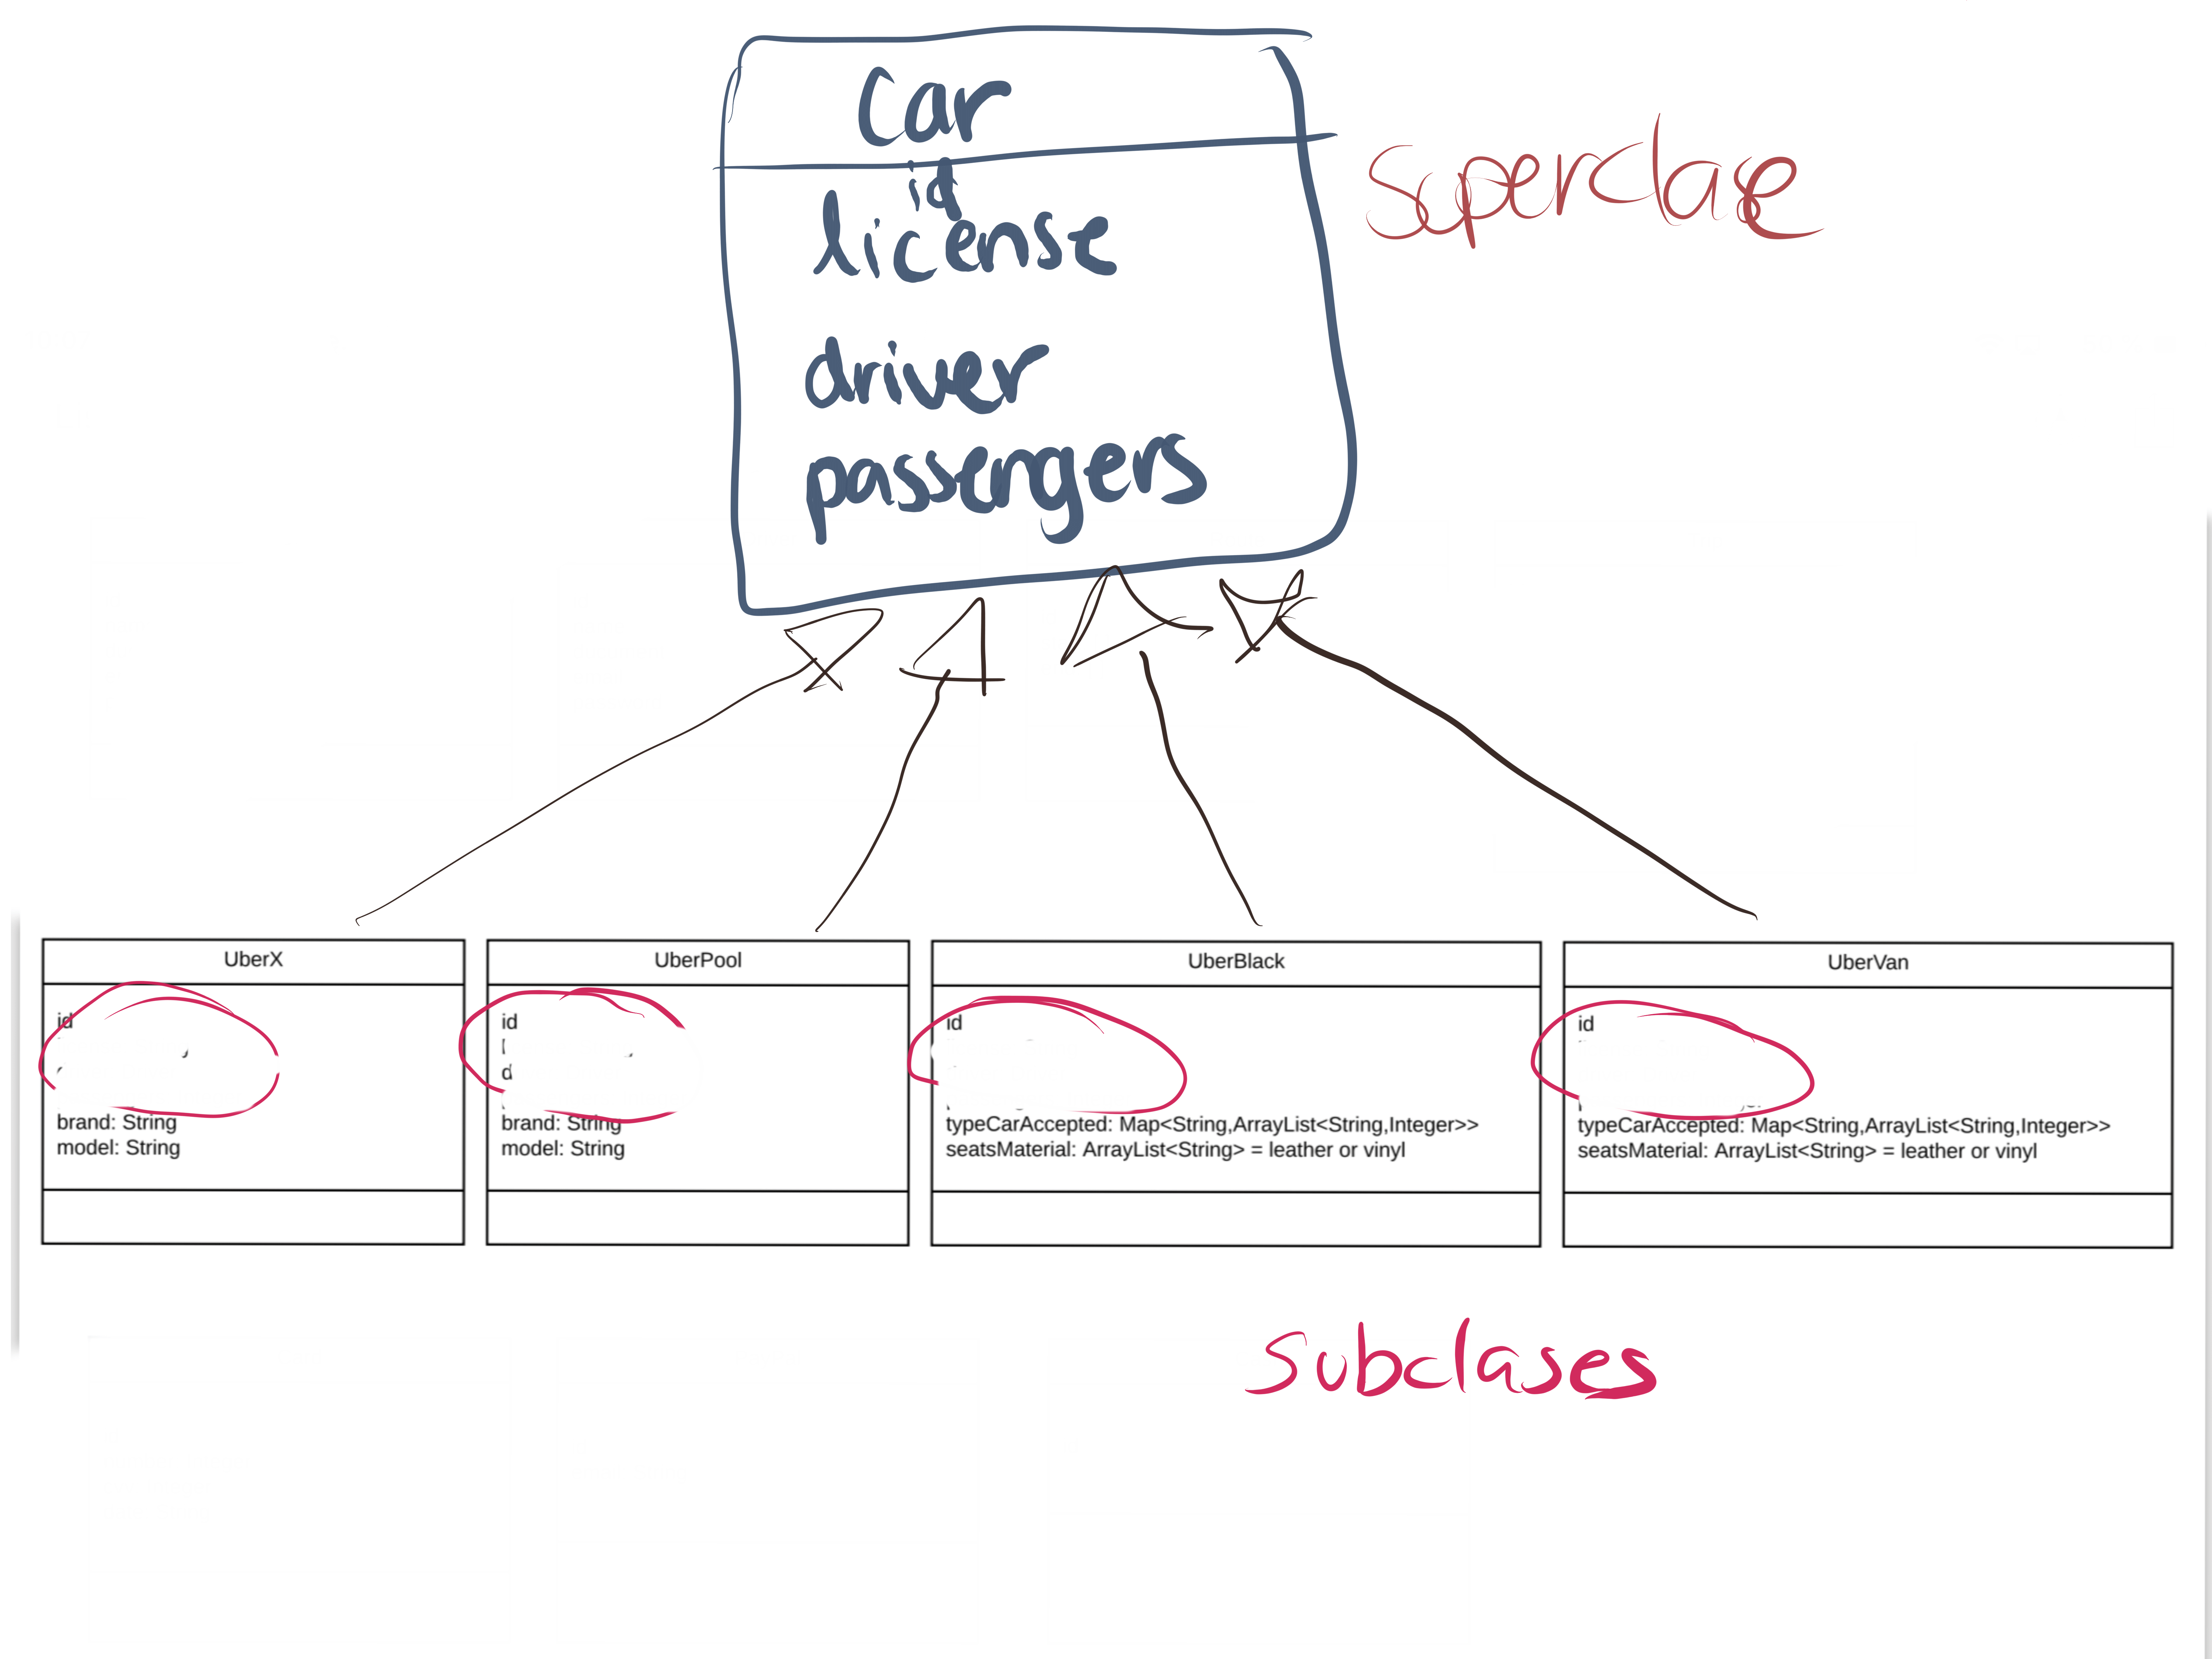
\includegraphics[scale=0.08]{./Pictures/016_herencia_proyecto_uber3.png}
\end{figure}

%% Clase 17 - Reto 2: analicemos un problema

\newpage
%% Clase 18
\section{Definiendo clases en Java y Python}%

\textbf{Main.java}
\begin{minted}{java}
  class Main {
    public static void main(String[] args) {
      System.out.println("Hola Mundo");
    }
  }
\end{minted}

\textbf{Account.java}
\begin{minted}{java}
  class Account {
    Integer id;
    String name;
    String document;
    String email;
    String password;
  }
\end{minted}

\textbf{Car.java}
\begin{minted}{java}
  class Car {
    Integer id;
    String license;
    String driver;
    Integer passenger;
  }
\end{minted}

\textbf{Payment.java}
\begin{minted}{java}
  class Payment {
    Integer id;
  }
\end{minted}

\textbf{Route.java}
\begin{minted}{java}
  import java.util.ArrayList;

  class Route {
    Integer id;
    ArrayList<Double> start;
    ArrayList<Double> end;
  }
\end{minted}

Ahora crearemos las clases en \textbf{Python}:\\

\textbf{main.py}
\begin{minted}{python}
  if __name__ == "__main__":
    print("Hola Mundo")
\end{minted}

\textbf{account.py}
\begin{minted}{python}
  class Account:
    id = int
    name = str
    document = str
    email = str
    password = str
\end{minted}

\textbf{car.py}
\begin{minted}{python}
  class Car:
    id = int
    license = str
    driver = str
    passenger = str
\end{minted}

\textbf{route.py}
\begin{minted}{python}
  class Route:
    id = int
    start = []
    end = []
\end{minted}

\textbf{payment.py}
\begin{minted}{python}
  class Payment:
    id = int
\end{minted}

%% Clase 19
\section{Definiendo clases en Javascript y PHP}%
En Javascript no existía como tal el concepto de clases hasta el nuevo estándar
EcmaScript 6. El reto de encontrar sistemas construidos con este estándar es
alto por esa razón te explicaré cuál fue por mucho tiempo su equivalente.\\

Los Prototipos fue la forma de crear clases en Javascript y las representaremos
partiendo de la declaración de una función.\\

Creemos nuestras clases:
\begin{itemize}
  \item Account
  \item Car
  \item Payment
  \item Route
\end{itemize}

Para esto crearemos el siguiente sistema de archivos dentro de la carpeta JS de
nuestro proyecto:

\begin{itemize}
  \item Account.js
  \item Car.js
  \item Payment.js
  \item Route.js
  \item index.js
\end{itemize}

El archivo index.js será el lugar equivalente al punto de entrada de la
aplicación donde estaremos declarando nuestros objetos basado en las clases.
Para esta clase lo dejaremos en blanco.\\

Ahora veamos el código archivo por archivo:\\

\textbf{Account.js}
\begin{minted}{javascript}
  function Account() {
    this.id;
    this.name;
    this.document;
    this.email;
    this.password;
  }
\end{minted}

\textbf{Car.js}
\begin{minted}{javascript}
  function Car() {
    this.id;
    this.license;
    this.driver;
    this.passenger;
  }
\end{minted}

\textbf{Payment.js}
\begin{minted}{javascript}
  function Payment() {
    this.id;
  }
\end{minted}

\textbf{Route.js}
\begin{minted}{javascript}
  function Route() {
    this.id;
    this.init;
    this.end;
  }
\end{minted}

Este es el enlace del codigo del proyecto:
\href{https://github.com/anncode1/Curso-POO-Platzi/tree/f5725787165b36cae579f94e428068039b554b0b/JS}{Enlace en Github.}

En este código notarás el uso de la palabra reservada this. Normalmente se usa
cuando usamos la sintaxis punto siempre lo haremos a partir de un objeto
instanciado, en este caso con this, se hace una simulación al objeto en
cuestión, a pesar de que en ese momento visualmente sigue siendo una clase.\\

Ahora crearemos las clases en PHP, para esto crearemos el siguiente sistema de
archivos dentro de la carpeta PHP de nuestro proyecto:

\begin{itemize}
  \item Account.php
  \item Car.php
  \item Payment.php
  \item Route.php
  \item index.php
\end{itemize}

\newpage
\textbf{Account.php}
\begin{minted}{php}
  <?php

  class Account {
    public $id;
    public $name;
    public $document;
    public $email;
    public $password;
  }

  ?>
\end{minted}

\textbf{Car.php}
\begin{minted}{php}
  <?php

  class Car {
    public $id;
    public $license;
    public $driver;
    public $passenger;
  }

  ?>
\end{minted}

\textbf{Payment.php}
\begin{minted}{php}
  <?php

  class Payment {
    public $id;
  }

  ?>
\end{minted}

\textbf{Route.php}
\begin{minted}{php}
  <?php

  class Route {
    public $id;
    public $init;
    public $end;
  }

  ?>
\end{minted}

\newpage
%% Clase 20
\section{Objetos, método constructor y su sintaxis en código}%
Los \textbf{objetos} nos ayudan a crear instancias de una clase, el objeto es el
resultado de lo que modelamos, de los parámetros declarados y usaremos los
objetos para que nuestras clases cobren vida.\\

Los \textbf{métodos constructores} dan un estado inicial al objeto y podemos
añadirle algunos datos al objeto mediante estos métodos. Los atributos o
elementos que pasemos a través del constructor serán los datos mínimos que
necesita el objeto para que pueda vivir.

Declarando un método constructor en:\\

\textbf{Java}

\begin{minted}{java}
  public Person(String name) {
    this.name = name;
  }
\end{minted}

\textbf{Python}

\begin{minted}{python}
  def __init__(self, name):
    self.name = name
\end{minted}

\textbf{JavaScript}

\begin{minted}{javascript}
  function Person(name) {
    this.name = name
  }
\end{minted}

\textbf{PHP}

\begin{minted}{php}
  public function_construct($name) {
    $this->name = name;
  }
\end{minted}

Instanciando un objeto usando el método constructor:
\textbf{Java}

\begin{minted}{java}
  Person person = new Person("Ann");
\end{minted}

\begin{minted}{python}
  person = Person("Ann")
\end{minted}


\begin{minted}{javascript}
  var person = new Person("Ann");
\end{minted}

\begin{minted}{php}
  $person = new Person("Ann");
\end{minted}


%%  Clase 21
\section{Objetos. Dando vida a nuestras clases en Java y Python}%

\textbf{Java}\\
Instanciamos objetos de tipo Car modificando nuestro archivo \textbf{Main.java}\\

\textbf{Main.java}
\begin{minted}{java}
  class Main {
    public static void main(String[] args) {
      System.out.println("Hola Mundo");
      Car car = new Car();
      car.licens = "AMQ123";
      car.driver = "Andres Herrera";
      car.passenger = 4;
      System.out.println("Car License: " + car.license);

      Car car2 = new Car();
      car2.license = "QWE567";
      car2.driver = "Andrea Herrera";
      car2.passenger = 3;
      System.out.println("Car License: " + car2.license);
    }
  }
\end{minted}

Ahora vamos agregar un método en la clase Car modificando el fichero \textbf{Car.java}\\

\textbf{Car.java}
\begin{minted}{java}
  class Car {
    Integer id;
    String license;
    String driver;
    Integer passenger;

    void printDataCar() {
      System.out.println("License: " + license + " Driver: " + driver);
    }
  }
\end{minted}


Con esto se reutiliza el código como podemos ver en el archivo \textbf{Main.java}\\

\textbf{Main.java}
\begin{minted}{java}
  class Main {
    public static void main(String[] args) {
      System.out.println("Hola Mundo");
      Car car = new Car();
      car.licens = "AMQ123";
      car.driver = "Andres Herrera";
      car.passenger = 4;
      car.printDataCar();

      Car car2 = new Car();
      car2.license = "QWE567";
      car2.driver = "Andrea Herrera";
      car2.passenger = 3;
      car2.printDataCar();
    }
  }
\end{minted}

\textbf{Python}\\
Ahora usando Python vamos a modificar el archivo \textbf{main.py}\\

\textbf{main.py}
\begin{minted}{python}
  from car import Car

  if __name__ == "__main__":
    print("Hola Mundo")
    car = Car()
    car.license = "AMS234"
    car.driver = "Andres Herrera"
    print(vars(car))

    car2 = Car()
    car2.license = "QWE567"
    car2.driver = "Martha"
    print(vars(car2))
\end{minted}
Como se observa, al imprimir los datos de un objeto en Python sin necesidad de
crear un método los despliega y en formato json.


%% Clase 22
\section{Declarando un Método Constructor en Java y JavaScript}%
Primero vamos arealizar los cambios en \textbf{Java}:\\
Vamos al fichero \textbf{Car.java} para escribir nuestro método constructor:\\

\textbf{Car.java}
\begin{minted}{java}
  class Car {
    Integer id;
    String license;
    Account driver;
    Integer passenger;

    public Car(String license, Account driver) {
      this.license = license;
      this.driver = driver;
    }

    void printDataCar() {
      System.out.println("License: " + license + "Name Driver: " + driver.name);
    }
  }
\end{minted}

También en nuestro método Account vamos a crear el método constructor
modificando el archivo \textbf{Account.java}\\

\textbf{Account.java}
\begin{minted}{java}
  class Account {
    Integer id;
    String name;
    String document;
    String email;
    String password;

    public Account(String name, String document) {
      this.name = name;
      this.document = document;
    }
  }
\end{minted}


Ahora en el archivo \textbf{Main.java} modificamos la instanciación de nuestros
objetos:\\

\textbf{Main.java}
\begin{minted}{java}
  class Main {
    public static void main(String[] args) {
      System.out.println("Hola Mundo");
      Car car = new Car("AMQ123", new Account("Andres Herrera", "AND123"));
      car.passenger = 4;
      car.printDataCar();

      Car car2 = new Car("QWE567", new Account("Andrea Herrera", "ANDA876"));
      car2.passenger = 3;
      car.printDataCar();
    }
  }
\end{minted}

Ahora vamos a realizar los mismos cambios en \textbf{JavaScript}.\\
Los resultados de un archivo en Javascript necesitan navegador para ser
visualizados. Por ello se va a crear un archivo \textbf{index.html} con el siguiente
contenido:\\

\textbf{index.html}
\begin{minted}{html}
  <!DOCTYPE html>
  <html lang="es">
  <head>
    <meta charset="UTF-8">
    <meta name="viewport" content="width=device-width, initial-scale=1.0">
    <meta http-equiv="X-UA-Compatible" content="ie=edge">
    <title>Document</title>
  </head>
  <body>
    <h1>Programación Orientada a Objetos en JavaScript</h1>
  </body>
  <script src="Account.js">
  <script src="Car.js">
  <script src="index.js"
  </html>
\end{minted}

Ahora cada vez que yo ejecute el sitio web \textbf{index.html} ejecutará
también el contenido del archivo \textbf{index.js}\\

\textbf{Car.js}
\begin{minted}{javascript}
  function Car(license, driver) {
    this.id;
    this.license = license;
    this.driver = driver;
    this.passenger;
  }

  Car.prototype.printDataCar = function () {
    console.log(this.driver)
    console.log(this.driver.name)
    console.log(this.driver.document)
  }
\end{minted}


\textbf{Account.js}
\begin{minted}{javascript}
  function Account(name, document) {
    this.id;
    this.name = name;
    this.document = document;
    this.email;
    this.password;
  }
\end{minted}


\textbf{index.js}
\begin{minted}{javascript}
  var car = new Car("AW456", new Account("Andres Herrera", "QWE234"))
  car.passenger = 4;
  car.printDataCar();
\end{minted}

%% Clase 23
\section{JavaScript orientado a objetos, lo más nuevo}%
A partir de las nuevas especificaciones del EcmaScript 6 ya podemos declarar
una clase con la palabra reservada \textit{class}, aunque es importante aclarar
que estos no dejan de ser prototipos, sino todo lo contrario.\\

Además tenemos una palabra clave para definir un constructor, y dentro de este
estarán las propiedades de nuestra clase definidas listas para inicializarse.\\

Transcribamos el código JavaScript que generamos en la clase anterior a este
nuevo estándar.\\

La clase \textbf{Car} quedaría así:

\begin{minted}{javascript}
  class Car {
    constructor(license, driver) {
      this.id;
      this.license = license;
      this.driver = driver;
      this.passenger;
    }

    printDataCar() {
      console.log(this.driver)
      console.log(this.driver.name)
      console.log(this.driver.document)
    }
  }
\end{minted}

Si quisiéramos declarar un método, en esta nueva sintaxis dejaremos de utilizar
la palabra clave \textit{function}.\\

Ahora veamos a la clase \textbf{Account}:\\

\textbf{Account.js}
\begin{minted}{javascript}
  class Account {
    constructor(name, document) {
      this.id;
      this.name = name;
      this.document = document;
      this.email;
      this.password;
    }
  }
\end{minted}

Y para finalizar aquí puedes ver las clases \textbf{Route} y \textbf{Payment}:\\

\textbf{Route.js}
\begin{minted}{javascript}
  class Route {
    constructor() {
      this.id;
      this.init;
      this.end;
    }
  }
\end{minted}

\textbf{Payment.js}
\begin{minted}{javascript}
  class Payment {
    constructor() {
      this.id;
    }
  }
\end{minted}

Notarás que para instanciar un objeto seguiremos usando la palabra clave \textit{new}.

\textbf{index.js}
\begin{minted}{javascript}
  var car = new Car("AW456", new Account("Andres Herrera", "QWE234"))
  car.passenger = 4;
  car.printDataCar();
\end{minted}

Y los resultados serán los mismos:

\begin{figure}[h!]
  \centering
  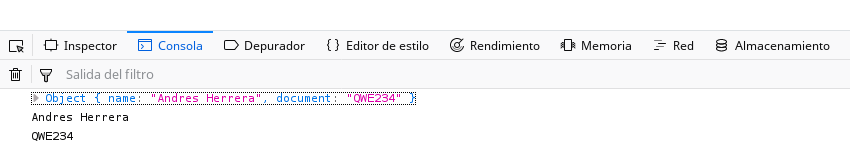
\includegraphics[scale=0.75]{./Pictures/017_objetos_js.png}
\end{figure}

%% Clase 24
\section{Declarando un Método Constructor en Python y PHP}%
En Python encontrarás un concepto denominado \textbf{Métodos Mágicos}, estos
métodos son llamados automáticamente y estrictamente bajo ciertas reglas. El
método constructor en Python forma parte de esta familia de métodos y como
aprendimos en la clase anterior lo declaramos usando {\_}{\_}init{\_}{\_},
aunque si nos ponemos estrictos este método no construye el objeto en sí. El
encargado de hacer esto es {\_}{\_}new{\_}{\_} y el método {\_}{\_}init{\_}{\_}
se encargará de personalizar la instaciación de la clase, esto significa que lo
que esté dentro de {\_}{\_}init{\_}{\_} será lo primero que se ejecute cuando
se cree un objeto de esta clase.

Para nuestro proyecto tenemos la necesidad de que algunas variables se
inicialicen obligatoriamente cuando ocurra la instanciación. Así que declaremos
el método {\_}{\_}init{\_}{\_} en las clases de nuestro proyecto con las
propiedades obligatorias.

Para la clase Account quedaría algo así, notarás que usamos la palabra clave
\textbf{self}, esta es muy parecida a lo que venimos trabajando a otros
lenguajes con \textbf{this}. Y como su nombre lo dice hace referencia a los
datos que componen la clase, en este caso \texttt{self.name} está llamando al
atributo name que se encuentra en la línea 3 de la clase y le está asignando el
dato que se pasa en el método {\_}{\_}init{\_}{\_}.\\

\textbf{account.py}
\begin{minted}{python}
  class Account:
    id = int
    name = str
    document = str
    email = str
    password = str

    def __init__(self, name, document):
      self.name = name
      self.document = document
\end{minted}

Ahora veamos la clase Car:\\

\textbf{car.py}
\begin{minted}{python}
  from account import Account

  class Car:
    id = int
    license = str
    driver = Account("", "")
    passenger = int

    def __init__(self, license, driver):
      self.license = license
      self.driver = driver
\end{minted}

Lo que notarás de diferente es que cambiamos el tipo de dato de
\textbf{driver}, ahora es de tipo Account y como ves está solicitando los dos
datos obligatorios para instancias un objeto de este tipo. Esto lo verás más en
acción en el próximo fragmento de código del archivo \textbf{main.py}.\\
Además, mucho ojo, en la primera línea observamos que es importante importar la
clase para poderla usar.\\

Nuestro archivo \textbf{main.py} ahora se verá así:\\

\textbf{main.py}
\begin{minted}{python}
  from car import Car
  from account import Account

  if __name__ == "__main__":
    print("Hola Mundo")

    car = Car("AMS234", Account("Andres Herrera", "ANDA876"))
    print(vars(car))
    print(vars(car.driver))
\end{minted}

Observa que estamos importando las dos clases que usaremos y las estamos
instanciando en los métodos constructores.\\

Los resultados serán los siguientes:

\begin{figure}[h!]
  \centering
  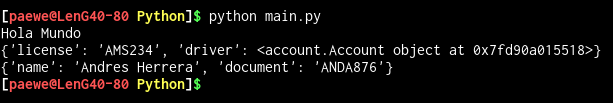
\includegraphics[scale=0.75]{./Pictures/018_resultado_python.png}
\end{figure}


Ahora trabajaremos \textbf{php}.\\

\textbf{Account.php}
\begin{minted}{php}
  <?php

  class Account {
    public $id;
    public $name;
    public $document;
    public $email;
    public $password;

    public function __construct($name, $document) {
      $this->name = $name;
      $this->document = $document;
    }
  }

  ?>
\end{minted}

\textbf{Car.php}
\begin{minted}{php}
  <?php

  include_once('Account.php');
  class Car {
    public $id;
    public $license;
    public $driver;
    public $passenger;

    public function __construct($license, Account $driver) {
      $this->license = $license;
      $this->driver = $driver;
    }

    public function printDataCar() {
      echo "License: $this->license Driver: ".$this->driver->name;
    }

  }

  ?>
\end{minted}

\textbf{index.php}
\begin{minted}{php}
  <?php

  include_once 'Car.php';
  $car = new Car("NNO23", new Account("Miguel", "PDI00008"));
  $car.printDataCar();
  echo "\n";

  ?>
\end{minted}

Los resultados serán los siguientes:

\begin{figure}[h!]
  \centering
  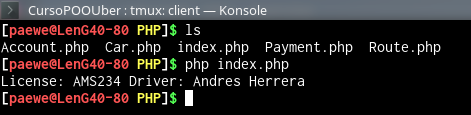
\includegraphics[scale=0.75]{./Pictures/019_resultado_php.png}
\end{figure}

%% Clase 25
\section{Aplicando herencia al lenguaje Java y PHP}%
La herencia se expresa dependiendo el lenguaje de programación que elijas:\\

\textbf{Java}
\begin{minted}{java}
  class Student extends Person
\end{minted}

\textbf{Python}
\begin{minted}{Python}
  class Student(Person):
\end{minted}

\textbf{JavaScript}
\begin{minted}{javascript}
  student.prototype = new Person();
\end{minted}

\textbf{PHP}
\begin{minted}{php}
  class Student extends Person
\end{minted}

Creamos un nuevo fichero en la carpeta Java llamado UberX.java\\

\textbf{UberX.java}
\begin{minted}{java}
  class UberX extends Car {
    String brand;
    String model;

    public UberX(String license, Account driver, String brand, String model) {
      super(license, driver);
      this.brand = brand;
      this.model = model;
    }
  }
\end{minted}

\textbf{UberPool.java}
\begin{minted}{java}
  class UberPool extends Car {
    String brand;
    String model;

    public UberPool(String license, Account driver, String brand, String model) {
      super(license, driver);
      this.brand = brand;
      this.model = model;
    }
  }
\end{minted}

\textbf{UberBlack.java}
\begin{minted}{java}
  import java.util.Map;
  import java.util.ArrayList;

  class UberBlack extends Car {
    Map<String, Map<String,Integer>> typeCarAccepted;
    ArrayList<String> seatsMaterial;

    public UberBlack(String license, Account driver,
    Map<String, Map<String,Integer>> typeCarAccepted,
    ArrayList<String> seatsMaterial) {
      super(license, driver);
      this.typeCarAcepted = typeCarAccepted;
      this.seatsMaterial = seatsMaterial;
    }
  }
\end{minted}

\textbf{UberVan.java}
\begin{minted}{java}
  class UberVan extends Car {
    Map<String, ArrayList<String,Integer>> typeCarAccepted;
    ArrayList<String> seatsMaterial;

    public UberVan(String license, Account driver,
    Map<String, ArrayList<String,Integer>> typeCarAccepted,
    ArrayList<String> seatsMaterial) {
      super(license, driver);
      this.typeCarAcepted = typeCarAccepted;
      this.seatsMaterial = seatsMaterial;
    }
  }
\end{minted}


Ahora vamos a ver como se hace en PHP. Igualmente creamos un nuevo archivo \textbf{uberX.php}\\

\textbf{uberX.php}
\begin{minted}{php}
  <?php
  require_once('car.php');
  class UberX extends Car {
    public $brand;
    public $model;

    public function __construct($license, $driver, $brand, $model) {
      parent::__construct($license, $driver);
      $this->brand = $brand;
      $this->model = $model;
    }
  }
  ?>
\end{minted}

\textbf{uberPool.php}
\begin{minted}{php}
  <?php
  require_once('car.php');
  class uberPool extends Car {
    public $brand;
    public $model;

    public function __construct($license, $driver, $brand, $model) {
      parent::__construct($license, $driver);
      $this->brand = $brand;
      $this->model = $model;
    }
  }
  ?>
\end{minted}

\textbf{uberBlack.php}
\begin{minted}{php}
  <?php
  require_once('car.php');

  class UberBlack extends Car {
    public $typeCarAccepted;
    public $seatsMaterial;

    public function __construct($license, $driver, $typeCarAccepted, $seatsMaterial) {
      parent::__construct($license, $driver);
      $this->typeCarAccepted = $typeCarAccepted;
      $this->seatsMaterial = $seatsMaterial;
    }
  }
  ?>
\end{minted}

\textbf{uberVan.php}
\begin{minted}{php}
  <?php
  require_once('car.php');

  class UberVan extends Car {
    public $typeCarAccepted;
    public $seatsMaterial;

    public function __construct($license, $driver, $typeCarAccepted, $seatsMaterial) {
      parent::__construct($license, $driver);
      $this->typeCarAccepted = $typeCarAccepted;
      $this->seatsMaterial = $seatsMaterial;
    }
  }
  ?>
\end{minted}


\textbf{main.php}
\begin{minted}{php}
  <?php

  require_once("car.php");
  require_once("uberX.php");
  require_once("uberPool.php");
  require_once("account.php");

  $uberX = new UberX("CVB123", new Account("Andres Herrera", "AND456"), "Chevrolet", "Spark");
  echo $uberX->printDataCar();
  echo "\n";

  $uberPool = new UberPool("TYU567", new Account("Andrea Ferran", "ANDA765"),
                           "Dodge", "Attitude");
  $uberPool->printDataCar();
  echo "\n";

  ?>
\end{minted}

%% Clase 26 - Solución del reto de herencia en PHP

%% Clase 27
\section{Aplicando herencia en lenguaje Python y JavaScript}%
\textbf{Python}\\

Recuerdas que en Python la herencia se expresa de manera muy similar a un
método constructor de otros lenguajes. Apliquemos herencia para nuestra familia
Car, para esto crearemos las siguientes clases:\\

\begin{itemize}
  \item UberX.py
  \item UberPool.py
  \item UberBlack.py
  \item UberVan.py
\end{itemize}

\textbf{uberX.py}
\begin{minted}{python}
  from car import Car

  class UberX(Car):
      brand = str
      model = str

      def __init(self, license, driver, brand, model):
          super.__init__(license, driver)
          self.brand = brand
          self.model = model
\end{minted}

\textbf{uberPool.py}
\begin{minted}{python}
  from car import Car

  class UberPool(Car):
      def __init__(self, license, driver, brand, model):
          super.__init__(license,driver)
          self.brand = brand
          self.model = model
\end{minted}

\textbf{uberBlack.py}
\begin{minted}{python}
  from car import Car

  class UberBlack(Car):
      typeCarAccepted = []
      seatsMaterial = []
      def __init__(self, license, driver, typeCarAccepted, seatsMaterial):
          super.__init__(license, driver)
          self.typeCarAccepted = typeCarAccepted
          self.seatsMaterial = seatsMaterial
\end{minted}

\textbf{uberVan.py}
\begin{minted}{python}
  from car import Car

  class UberVan(Car):
      typeCarAccepted = []
      seatsMaterial = []

      def __init__(self, license, driver, typeCarAccepted, seatsMaterial):
          super.__init__(license, driver)
          self.typeCarAccepted = typeCarAccepted
          self.seatsMaterial = seatsMaterial
\end{minted}

\textbf{JavaScript}\\
En clases anteriores te expliqué cómo ejecutar herencia en estándares
anteriores al EcmaScript 6. Uno de los beneficios de utilizar este nuevo
estándar es el ejecutar herencia tan simple como utilizar la palabra reservada
\textbf{extends}.\\

\textbf{UberX.js}
\begin{minted}{javascript}
  class UberX extends Car {
    constructor(license, driver, brand, model) {
      super(license, driver)
      this.brand = brand;
      this.model = model;
    }
  }
\end{minted}

\textbf{UberPool.js}
\begin{minted}{javascript}
  class UberPool extends Car {
    constructor(license, driver, brand, model) {
      super(license, driver)
      this.brand = brand;
      this.model = model;
    }
  }
\end{minted}

\textbf{UberBlack.js}
\begin{minted}{javascript}
  class UberBlack extends Car {
    constructor(license, driver, typeCarAccepted, seatsMaterial) {
      super(license, driver)
      this.typeCarAccepted = typeCarAccepted;
      this.seatsMaterial = seatsMaterial;
    }
  }
\end{minted}

\textbf{UberVan.js}
\begin{minted}{javascript}
  class UberVan extends Car {
    constructor(license, driver, typeCarAccepted, setasMaterial) {
      super(license, driver)
      this.typeCarAccepted = typeCarAccepted;
      this.seatsMaterial = seatsMaterial;
    }
  }
\end{minted}

Ahora para utilizar una de las clases y crear un objeto, por ejemplo de UberX
no olvides declarar la clase en el archivo \textbf{index.html}\\

\textbf{index.html}
\begin{minted}{html}
  <!DOCTYPE html>
  <html lang="es">
    <head>
      <meta charset="utf-8">
      <meta name="viewport" content="width=device-width, initial-scale=1.0">
      <meta http-equiv="X-UA-Compatible" content="ie=edge">
      <title>Document</title>
    </head>
    <body>
      <h1>Programación Orientada a Objetos en JavaScript</h1>
    </body>
    <script src="Account.js" charset="utf-8"></script>
    <script src="Car.js" charset="utf-8"></script>
    <script src="UberX.js" charset="utf-8"></script>
    <script src="index.js" charset="utf-8"></script>
  </html>
\end{minted}

Nuestro ejemplo se verá así:\\

\textbf{index.js}
\begin{minted}{javascript}
  var car = new Car("AW456", new Account("Andres Herrera", "QWE234"))
  car.passenger = 4;
  car.printDataCar();

  var uberX = new UberX("QWE567", new Account("Andrea Ferran", "ANDA765"), "Chevrolet", "Spark")
  uberX.passenger = 4;
  uberX.printDataCar();
\end{minted}

%% Clase 28
\section{Otros tipos de Herencia}%
A partir de ahora las clases que estén siendo heredadas las llamaremos
familias.\\

Acabamos de aplicar herencia a la familia \textbf{Car}. Ahora apliqu'emosla a
la familia \textbf{Payment}.\\

En clases anteriores te mencioné que otro punto de partida que puedes tomar
para aplicar herencia es del hecho de que hay clases que lógicamente deberían
estar en una familia como es el caso de Payment.\\

\begin{figure}[h!]
  \centering
  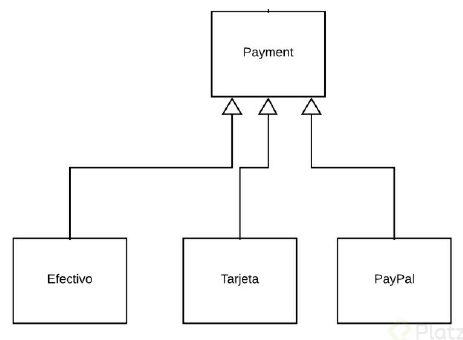
\includegraphics[scale=0.75]{./Pictures/020_otros_tipos_herencia.png}
\end{figure}

Notarás que a nivel de código parece inservible pero cuando estemos en el caso
de uso Pagar un Viaje, probablemente en ese momento sabremos cuál es el método
de pago, y necesitamos ingresar un dato lo suficientemente genérico que
conceptualmente nos de la información que necesitamos, en este caso que es un
Payment. Este es un tipo de Polimorfismo y uno de los principios SOLID del
software que obedece a la Inyección de Dependencias. Lo veremos más adelante a
detalle.\\

Ahora nos faltará crear las clases y aplicar su herencia.


%% Clase 29 - Reto 4:

%% Clase 30
\section{Encapsulamiento}%
El \textbf{Encapsulameinto} es hacer que un dato sea inviolable, inalterable
cuando se le asigne un modificador de acceso.\\

Para que un dato permanezca inviolable, inalterable, se le asigna un
modificador de acceso.\\

\begin{figure}[h!]
  \centering
  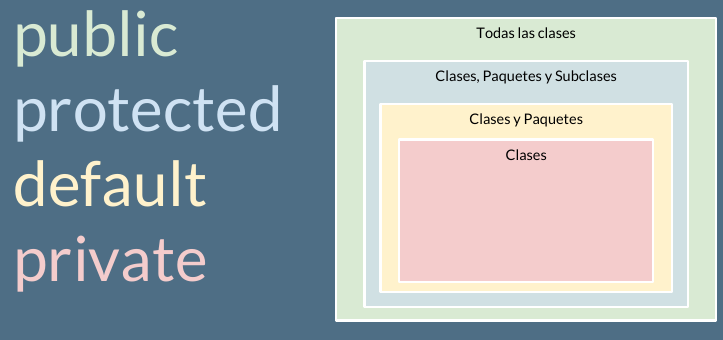
\includegraphics[scale=0.75]{./Pictures/021_encapsulamiento.png}
\end{figure}

%% Clase 31
\section{Encapsulando atributos en Java}%
Hay atributos que no se deben poder modificar de manera directa desde la clase
Main de nuestra aplicación y en el caso de nuestro proyecto Uber el atributo
\textbf{passenger} de la clase \textbf{Car} es un ejemplo, queremos que este
atributo tenga asignado el valor 4. Vamos a encapsular este atributo, pero
luego de hacerlo no significa que no podremos acceder a este atributo sino que
podremos hacerlo a través de métodos disponibles en muchos lenguajes y por
supuesto en java llamados \textbf{Getters y Setters} que nos permiten obtener
sus valores y asignarles respectivamente.\\

\textbf{Car.java}
\begin{minted}{java}
  class Car {
      Integer id;
      private String license;
      private Account driver;
      private Integer passenger;

      public Car(String license, Account driver) {
          this.license = license;
          this.driver = driver;
      }

      void printDataCar() {
          System.out.println("License: " + license + " Driver: " + driver.name +
                             " Passengers: " + passenger);
      }

      public Integer getPassenger() {
          return passenger;
      }

      public void setPassenger(Integer passenger) {
        this.passenger = passenger;
      }
  }
\end{minted}

Como se observa dentro del método \textbf{setPassenger} tenemos un condicional
que permite asignar el valor 4 a la variable passenger y en caso no se intente
ingresar ese valor entonces no se asigna y despliega un mensaje. De esta manera
se tiene mayor control gracias al encapsulamiento\\

%% Clase 32
\section{Generando Polimorfismo en Java}%
Polimorfismo: Muchas formas. Poli = muchas, morfismo = formas. No es Poliformismo.\\
Es construir con el mismo nombre pero con comportamiento diferente.

Por ejemplo en nuestro proyecto vamos a crear polimorfismo del setter
\textbf{setPassenger} para la subclase UberVan, para ello modificamos los siguiente fichero:

\textbf{UberVan.java}
\begin{minted}{java}
  import java.util.ArrayList;
  import java.util.Map;

  class UberVan extends Car {
      Map<String, Map<String,Integer>> typeCarAccepted;
      ArrayList<String> seatsMaterial;

      public UberVan(String license, Account driver) {
          super(license, driver);
      }

      @Override
      public void setPassenger(Integer passenger) {
          if (passenger == 6) {
              super.setPassenger(passenger);
          } else {
              System.out.println("Necesitas asignar 6 pasajeros");
          }
      }
  }
\end{minted}

\textbf{UberBlack.java}
\begin{minted}{java}
  import java.util.Map;
  import java.util.ArrayList;

  class UberBlack extends Car {
      Map<String, Map<String,Integer>> typeCarAccepted;
      ArrayList<String> seatsMaterial;

      public UberBlack(String license, Account driver,
                       Map<String, Map<String,Integer>> typeCardAccepted,
                       ArrayList<String> seatsMaterial) {
          super(license, driver);
          this.typeCarAccepted = typeCardAccepted;
          this.seatsMaterial = seatsMaterial;
      }

      @Override
      public void setPassenger(Integer passenger) {
          if(passenger == 4) {
              super.setPassenger(passenger);
          } else {
              System.out.println("Necesitas asignar 4 pasajeros");
          }
      }
  }
\end{minted}

\textbf{UberX.java}
\begin{minted}{java}
  class UberX extends Car {
      String brand;
      String model;

      public UberX(String license, Account driver, String brand, String model) {
          super(license, driver);
          this.brand = brand;
          this.model = model;
      }

      @Override
      public void setPassenger(Integer passenger) {
          if(passenger == 4) {
              super.setPassenger(passenger);
          } else {
              System.out.println("Necesitas asignar 4 pasajeros");
          }
      }
  }
\end{minted}

\textbf{UberPool.java}
\begin{minted}{java}
  class UberPool extends Car {
      String brand;
      String model;

      public UberPool(String license, Account driver, String brand, String model) {
          super(license, driver);
          this.brand = brand;
          this.model = model;
      }

      @Override
      public void setPassenger(Integer passenger) {
          if(passenger == 4) {
              super.setPassenger(passenger);
          } else {
              System.out.println("Necesitas asignar 4 pasajeros");
          }
      }
  }
\end{minted}



\textbf{Main.java}
\begin{minted}{java}
  class Main {
      public static void main(String[] args) {
          System.out.println("Hola mundo");
          UberX uberX = new UberX("AMQ123", new Account("Andres Herrera", "AND123"),
                                  "Chevrolet", "Sonic");
          uberX.setPassenger(4);
          uberX.printDataCar();

          UberVan uberVan = new UberVan("FGH345", new Account("Andrea Ferrol", "ANDA765"));
          uberVan.setPassenger(6);
          uberVan.printDataCar();
      }
  }
\end{minted}

%% Clase 33
\section{El Diagrama UML de Uber}%
Este es el diagrama que finalmente obtuvimos, aquí solo faltaría añadirle los
atributos que posee cada clase.

\begin{figure}[h!]
  \centering
  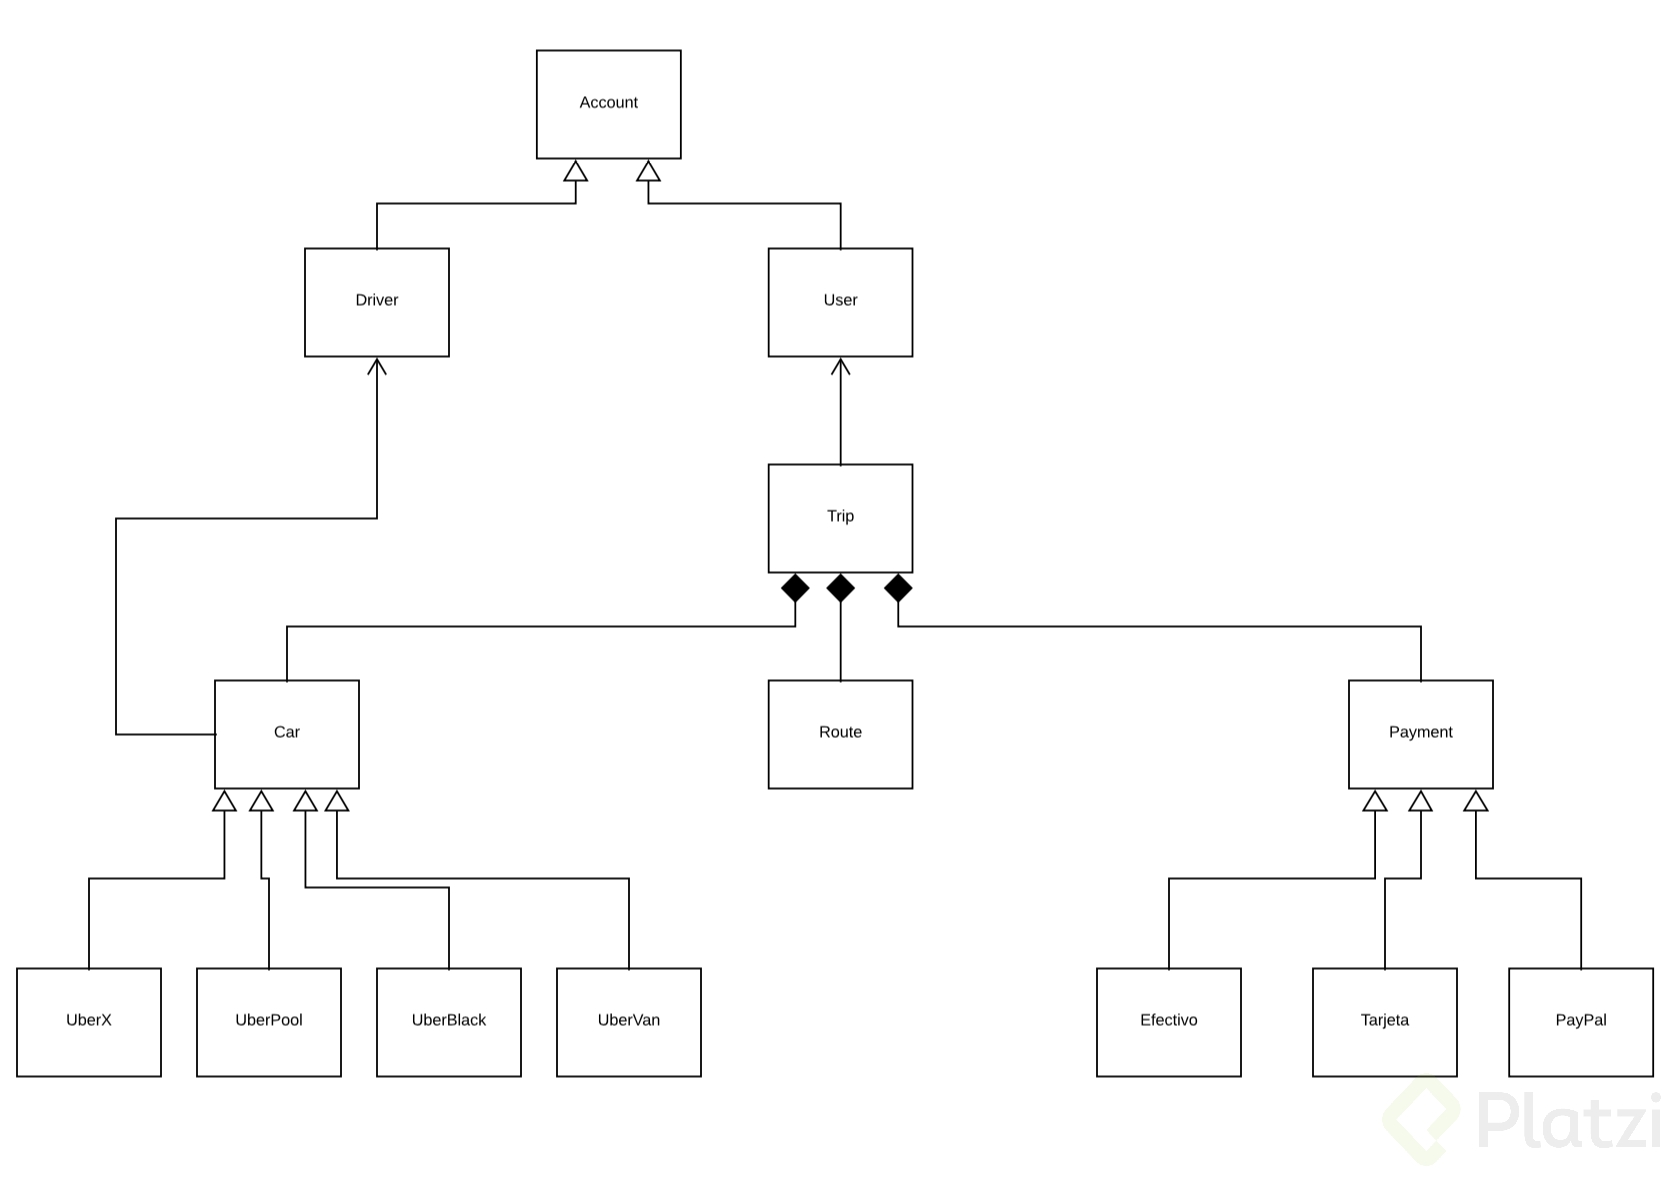
\includegraphics[scale=0.25]{./Pictures/033_uml_Uber.jpg}
\end{figure}




\vspace{2cm}
\LARGE\textit{RuneCode}


\end{document}

